\section{ПОИСК ОПТИМАЛЬНОЙ МОДЕЛИ}
В области исследований генеративных моделей преобладание больших моделей привело к проблемам при проведении исследований и анализе их производительности. Размер модели напрямую влияет на вычислительные требования и возможности исследователя. соотношение размера модели и ее качества является важным фактором при выборе модели.

На сегодняшний день существует ряд сложных наборов данных, предназначенных для оценки знаний, полученных моделями в процессе предварительного обучения. Один из таких наборов данных, известный как <<\textit{Massive Multitask Language Understanding}>> (MMLU) \cite{MMLU-bench}, является особенно сложным и требует обширного знания от моделей, полученных во время предварительного обучения, на различных задачах. Этот датасет включает задачи с разной степенью сложности, от простых до профессиональных. На данный момент наиболее оптимальной моделью на этом наборе данных является Flan-T5-XL с 3 миллиардами параметров, имея результат $52.4\%$. Еще одной моделью, которая может составить ей конкуренцию, является LLAMA-13B c результатом $46.9\%$, но ее большой размер делает процесс обучения значительно более затратным по сравнению с Flan-T5-XL.

Flan-T5 является моделью семейства T5, добавляя в дообучающую выборку большое количество инструкций, что позволило значительно улучшить качество модели на новых задачах.

\section{ПОИСК ОПТИМАЛЬНЫХ ГИПЕРПАРАМЕТРОВ ДЛЯ МОДЕЛИ}
\subsection{ПОСТАНОВКА ЗАДАЧИ}

Из гиперпараметров, значетельно влияющих на процесс обучения модели, было выделено две группы:
\begin{enumerate}
  \item Планировщики скорости обучения:
        \begin{itemize}
          \item константный;
          \item константный с прогревом;
          \item линейный;
          \item косинусный;
          \item косинусный с перезагрузками;
          \item полиномиальный;
          \item обратный квадратный корень.
        \end{itemize}
  \item Скорость обучения $\eta \in \{1 \times 10^{-4}, 2 \times 10^{-4}, \ldots, 9 \times 10^{-4}, 1 \times 10^{-3}\}$.
\end{enumerate}

\subsubsection{МЕТРИКИ ОЦЕНКИ КАЧЕСТВА ГЕНЕРАЦИИ МОДЕЛЕЙ}

Оценка качества генерации моделей явялется сложной задачей и малоисследованной. В данной работе помимо значений функции ошибки на валидационных данных используются метрики Exact Match и MAUVE \cite{mauve-paper}, позволяющие сравнивать гиперпараметры между собой. Модель обучалась с различными гиперпараметрами в группе, пока остальные гиперпараметры фиксировались.

Метрика Exact Match показывает, какой процент фраз при генерации совпал с ожидаемыми, а MAUVE подсчитывает то, насколько совпало распределение вероятностей сгенерированных фраз с распределением вероятностей ожидаемых фраз, суммируя ошибки первого и второго типа с использованием расхождения Куллбэка-Лейблера (KL).

Чтобы посчитать метрику MAUVE требуется получить два распределения вероятности возникновения токенов в генерируемой и ожидаемой последовательностях: $Q$ и $P$ соответственно. На основе этих распределений можно получить ошибки первого и второго рода, использовав KL как:
\begin{enumerate}
  \item Ошибка первого рода, когда генерируемое распределение $Q$ маловероятно при ожидаемом распределении $P$: $\text{KL}(Q \vert P)$.
  \item Ошибка второго рода, когда $Q$ не может сгенерировать текст, который правдоподобен при $P$: $\text{KL}(P \vert Q)$.
\end{enumerate} Расхождение Куллбэка-Лейблера определяется как:
\begin{equation}
  \text{KL}(Q \vert P) = \sum_{x \in \mathbf{x}}{Q(x) \log{\frac{Q(x)}{P(x)}}}.
\end{equation}

Из-за того, что распределения $Q$, $P$ могут быть неидентичны, то $\text{KL}(P \vert Q)$ или $\text{KL}(Q \vert P)$ может быть бесконечным, что делает неудобным использование $\text{KL}(P \vert Q)$ и $\text{KL}(Q \vert P)$ в качестве метрики. Для решения этой проблемы ошибки первого и второго рода учитываются в совместном распределении: 
\begin{equation}
  R_{\alpha} = \alpha P + (1 - \alpha)Q,
\end{equation} где $\alpha \in (0, 1)$ -- доверительный интервал.

С использованием совместного распределения $R_{\alpha}$ строится кривая расхождения $\mathcal{C}(P, Q)$, определяемая как:
\begin{equation}
  \mathcal{C}(P, Q) = \{\left(\exp[-c\text{KL}(Q \vert R_{\alpha})], \exp[-c\text{KL}(P \vert R_{\alpha})]\right)\},
\end{equation}где $c > 0$ -- поправочный коэффициент.

Посчитав область под $\mathcal{C}(P, Q)$, получим значение метрики MAUVE.

\subsection{АНАЛИЗ РЕЗУЛЬТАТОВ ЭКСПЕРИМЕНТОВ С ГИПЕРПАРАМЕТРАМИ}

При стартовой скорости обучения $\eta = 1 \times 10^{-3}$ на ограниченном наборе данных были произведены эксперименты по поиску оптимального планировщика скорости обучения $\varsigma$. В процессе экспериментов отметим, что планировщик с обратным квадратным корнем не представлен на графиках, так как ни один из запусков эксперимента с использованием этого планировщика не был успешно завершен.

В ходе экспериментов большинство планировщиков не оказало заметного влияния на скорость обучения и метрики. Среди рассмотренных вариантов планировщиков, в среднем наилучшие результаты продемонстрировал константный планировщик. Наименее эффективным, но успешно завершившим процесс обучения, оказался линейный планировщик. Отметим, что линейный планировщик характеризуется низким начальным значением функции ошибки на тренировочных и показывает наихудшие конечные значения на метрике MAUVE, что иллюстрируется на рисунках \ref{lr-s-train-loss} и \ref{lr-s-mauve}. График изменения скорости обучения представлен на рисунке \ref{lr-s-lr}. Ход экспериментов можно наблюдать на рисунках \ref{lr-s-train-loss}, \ref{lr-s-eval-loss}, \ref{lr-s-em}, \ref{lr-s-mauve}

% LR SCHEDULER
\begin{figure}[H]
  \centering
  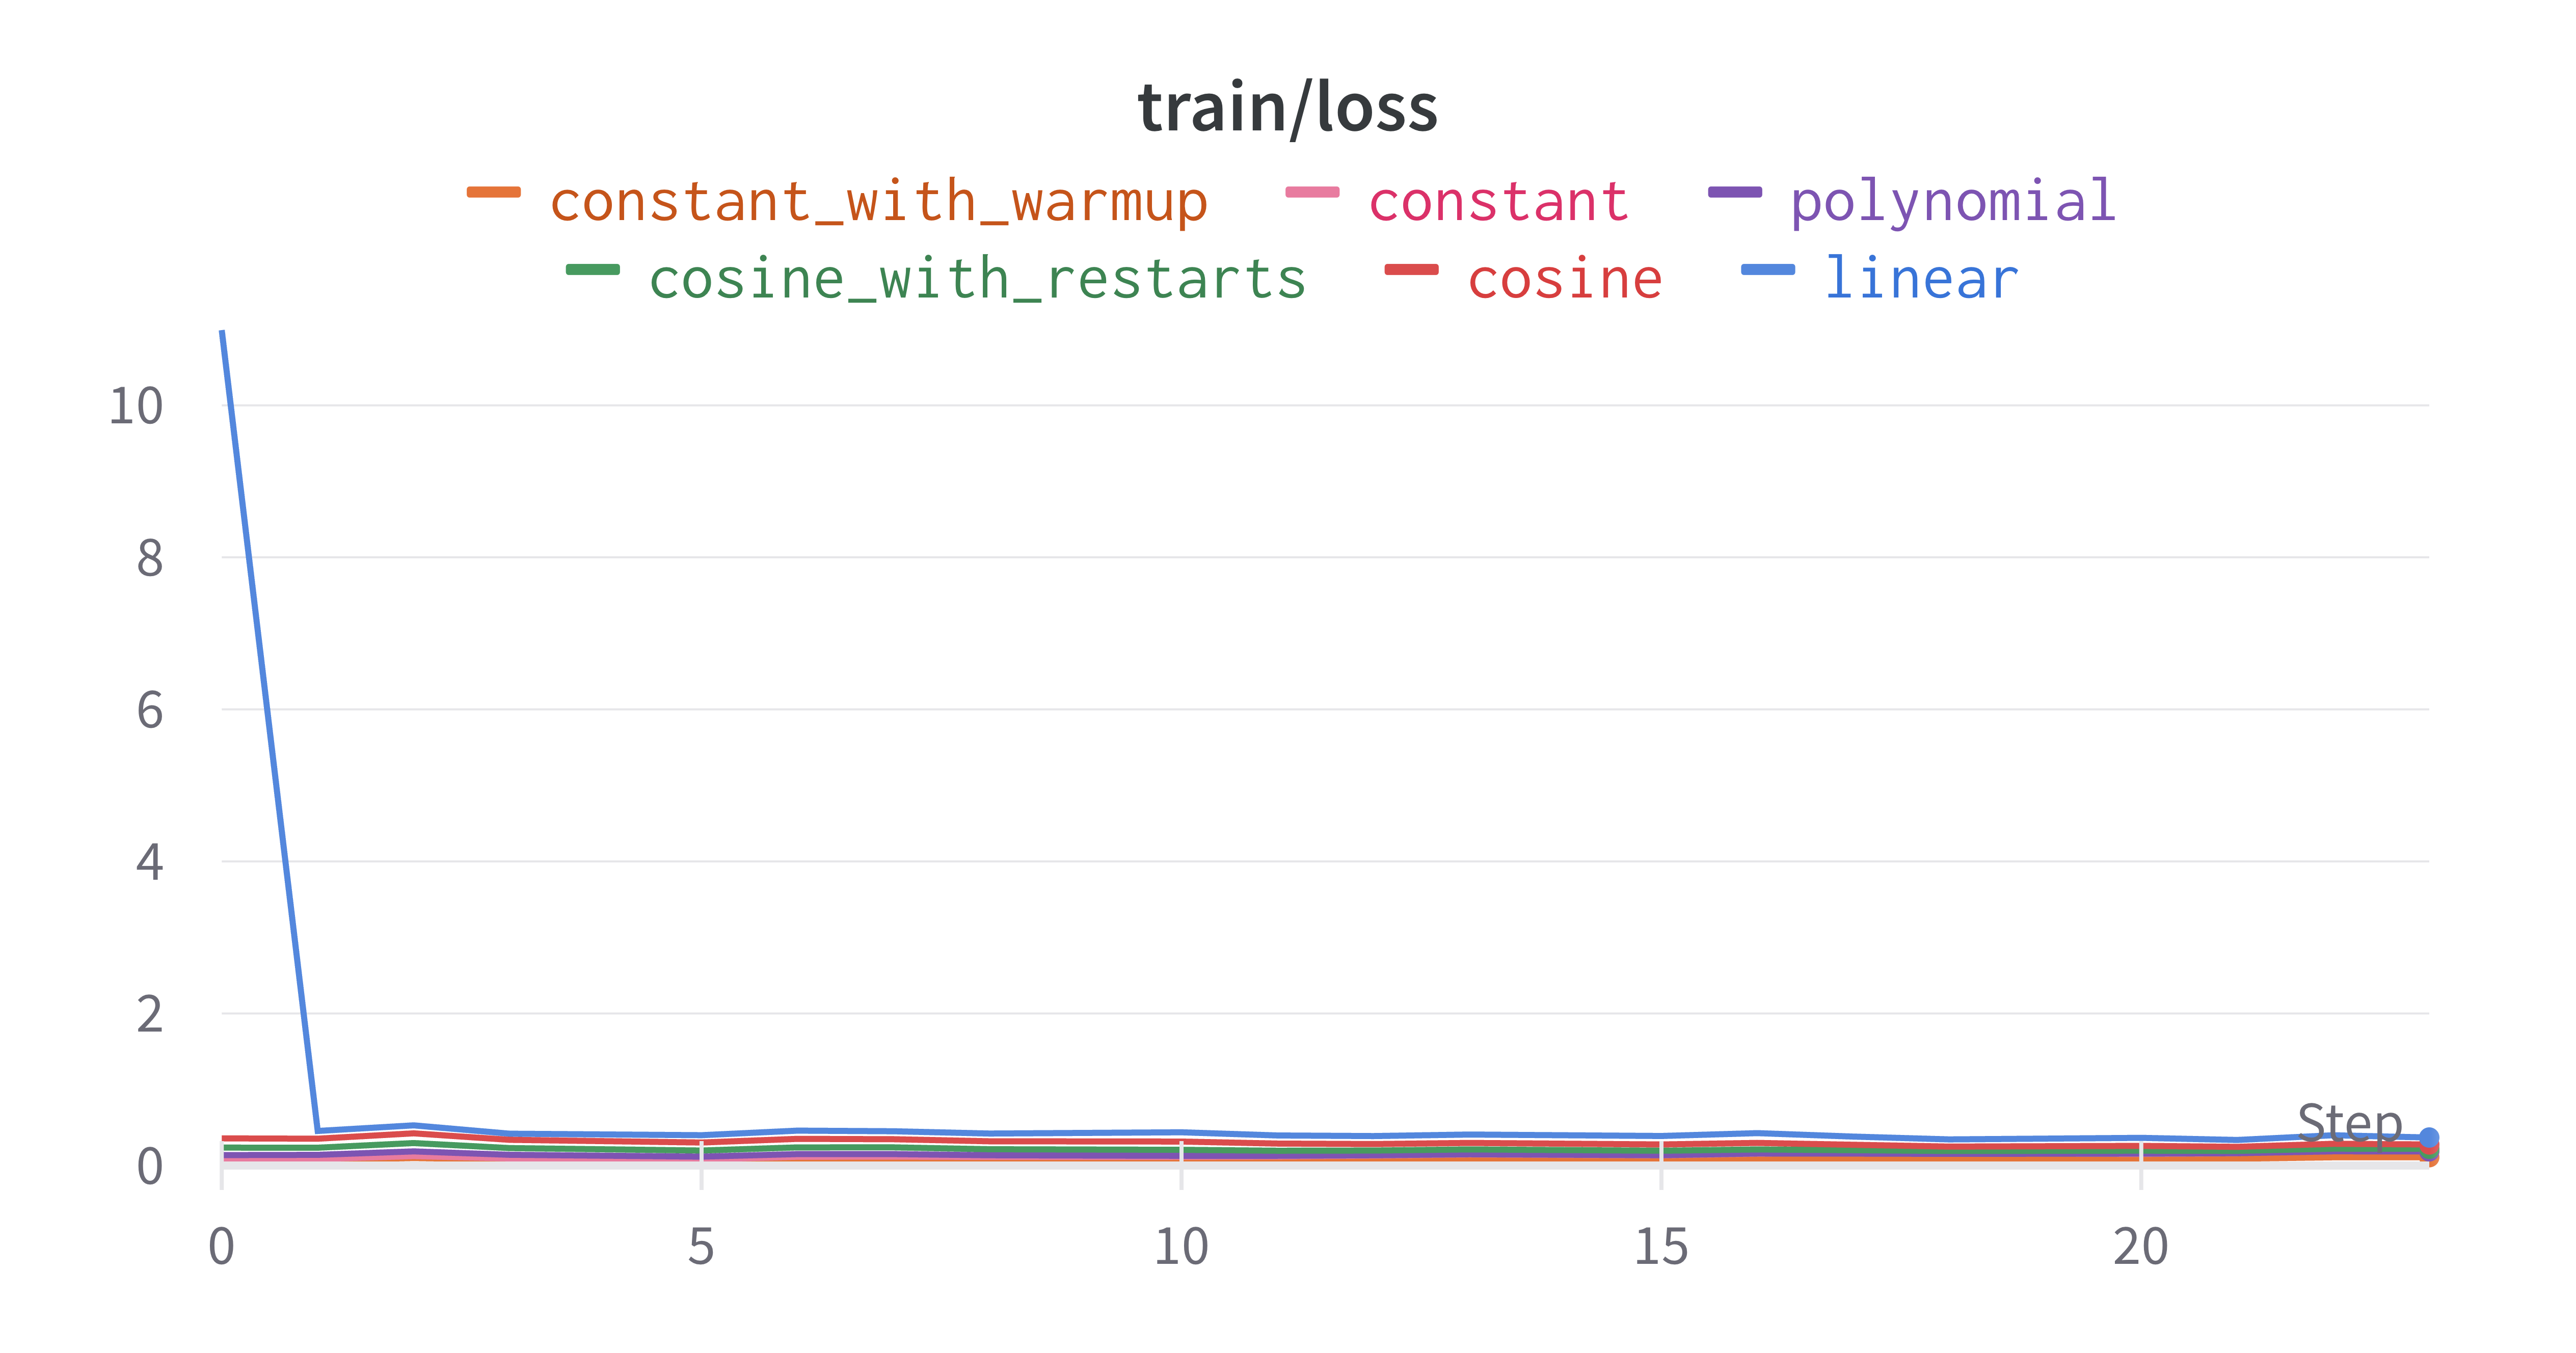
\includegraphics[width=.6\textwidth]{lr-s-train-loss}
  \caption{Значение функции ошибки на тренировочных данных}
  \label{lr-s-train-loss}
\end{figure}

\begin{figure}[H]
  \centering
  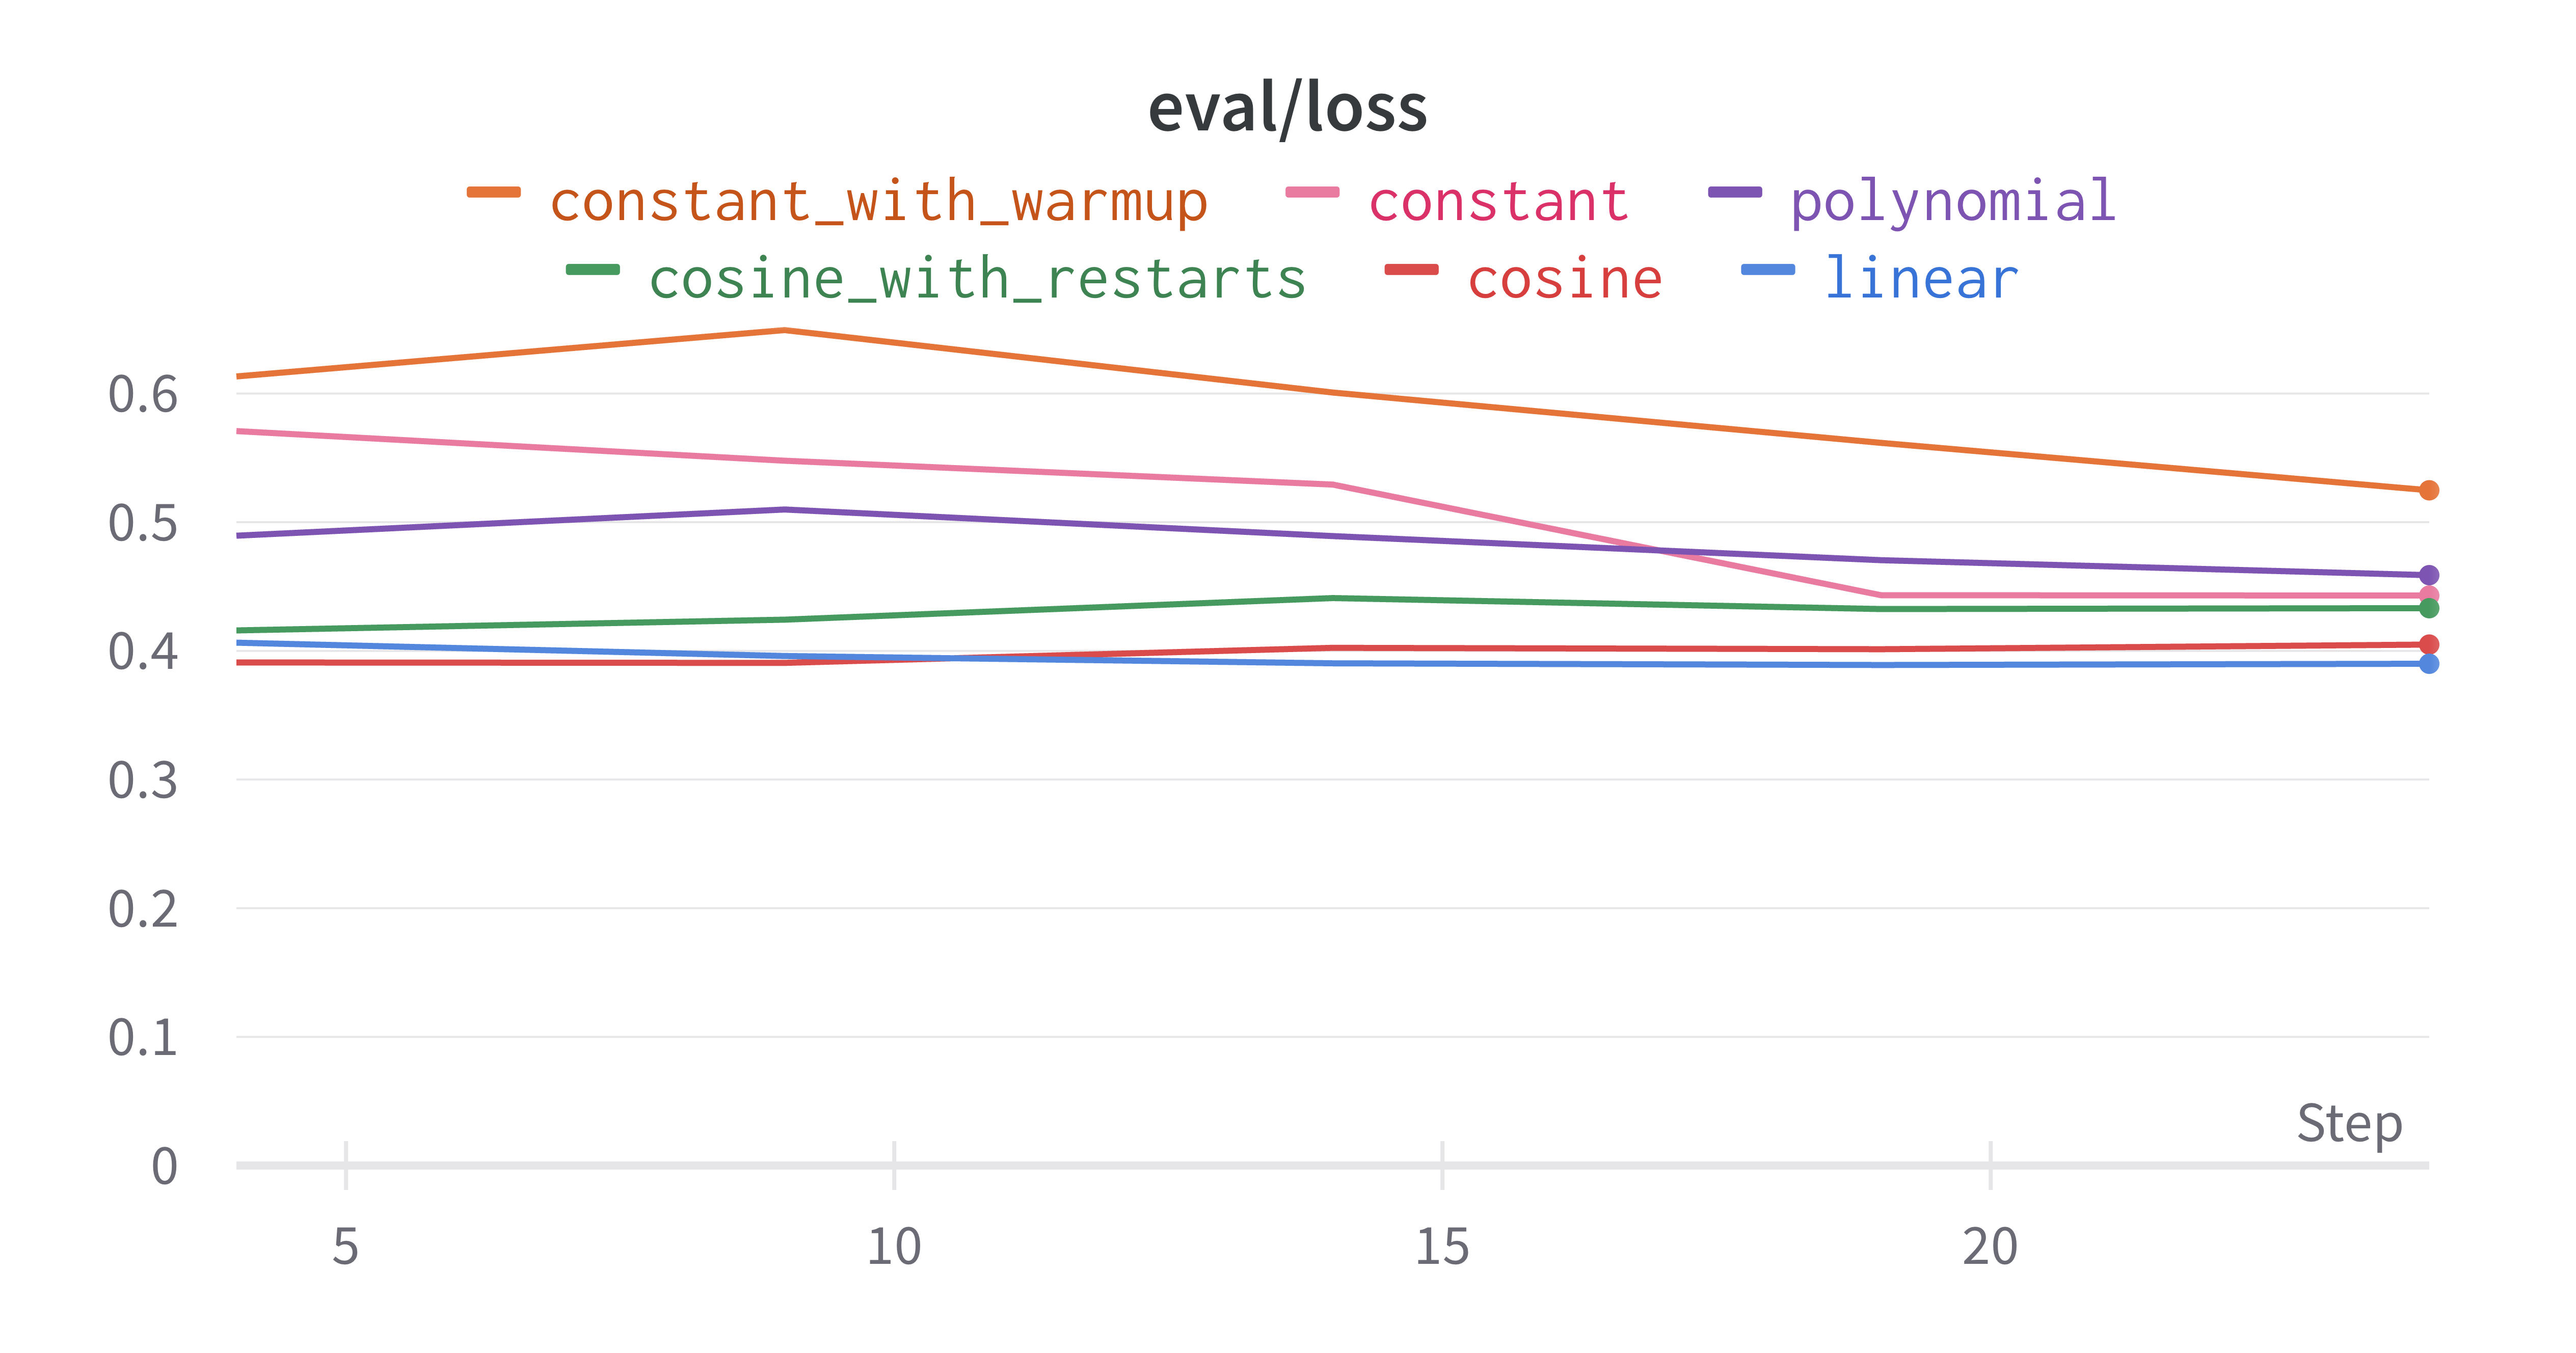
\includegraphics[width=.6\textwidth]{lr-s-eval-loss}
  \caption{Значение функции ошибки на валидационных данных}
  \label{lr-s-eval-loss}
\end{figure}

\begin{figure}[H]
  \centering
  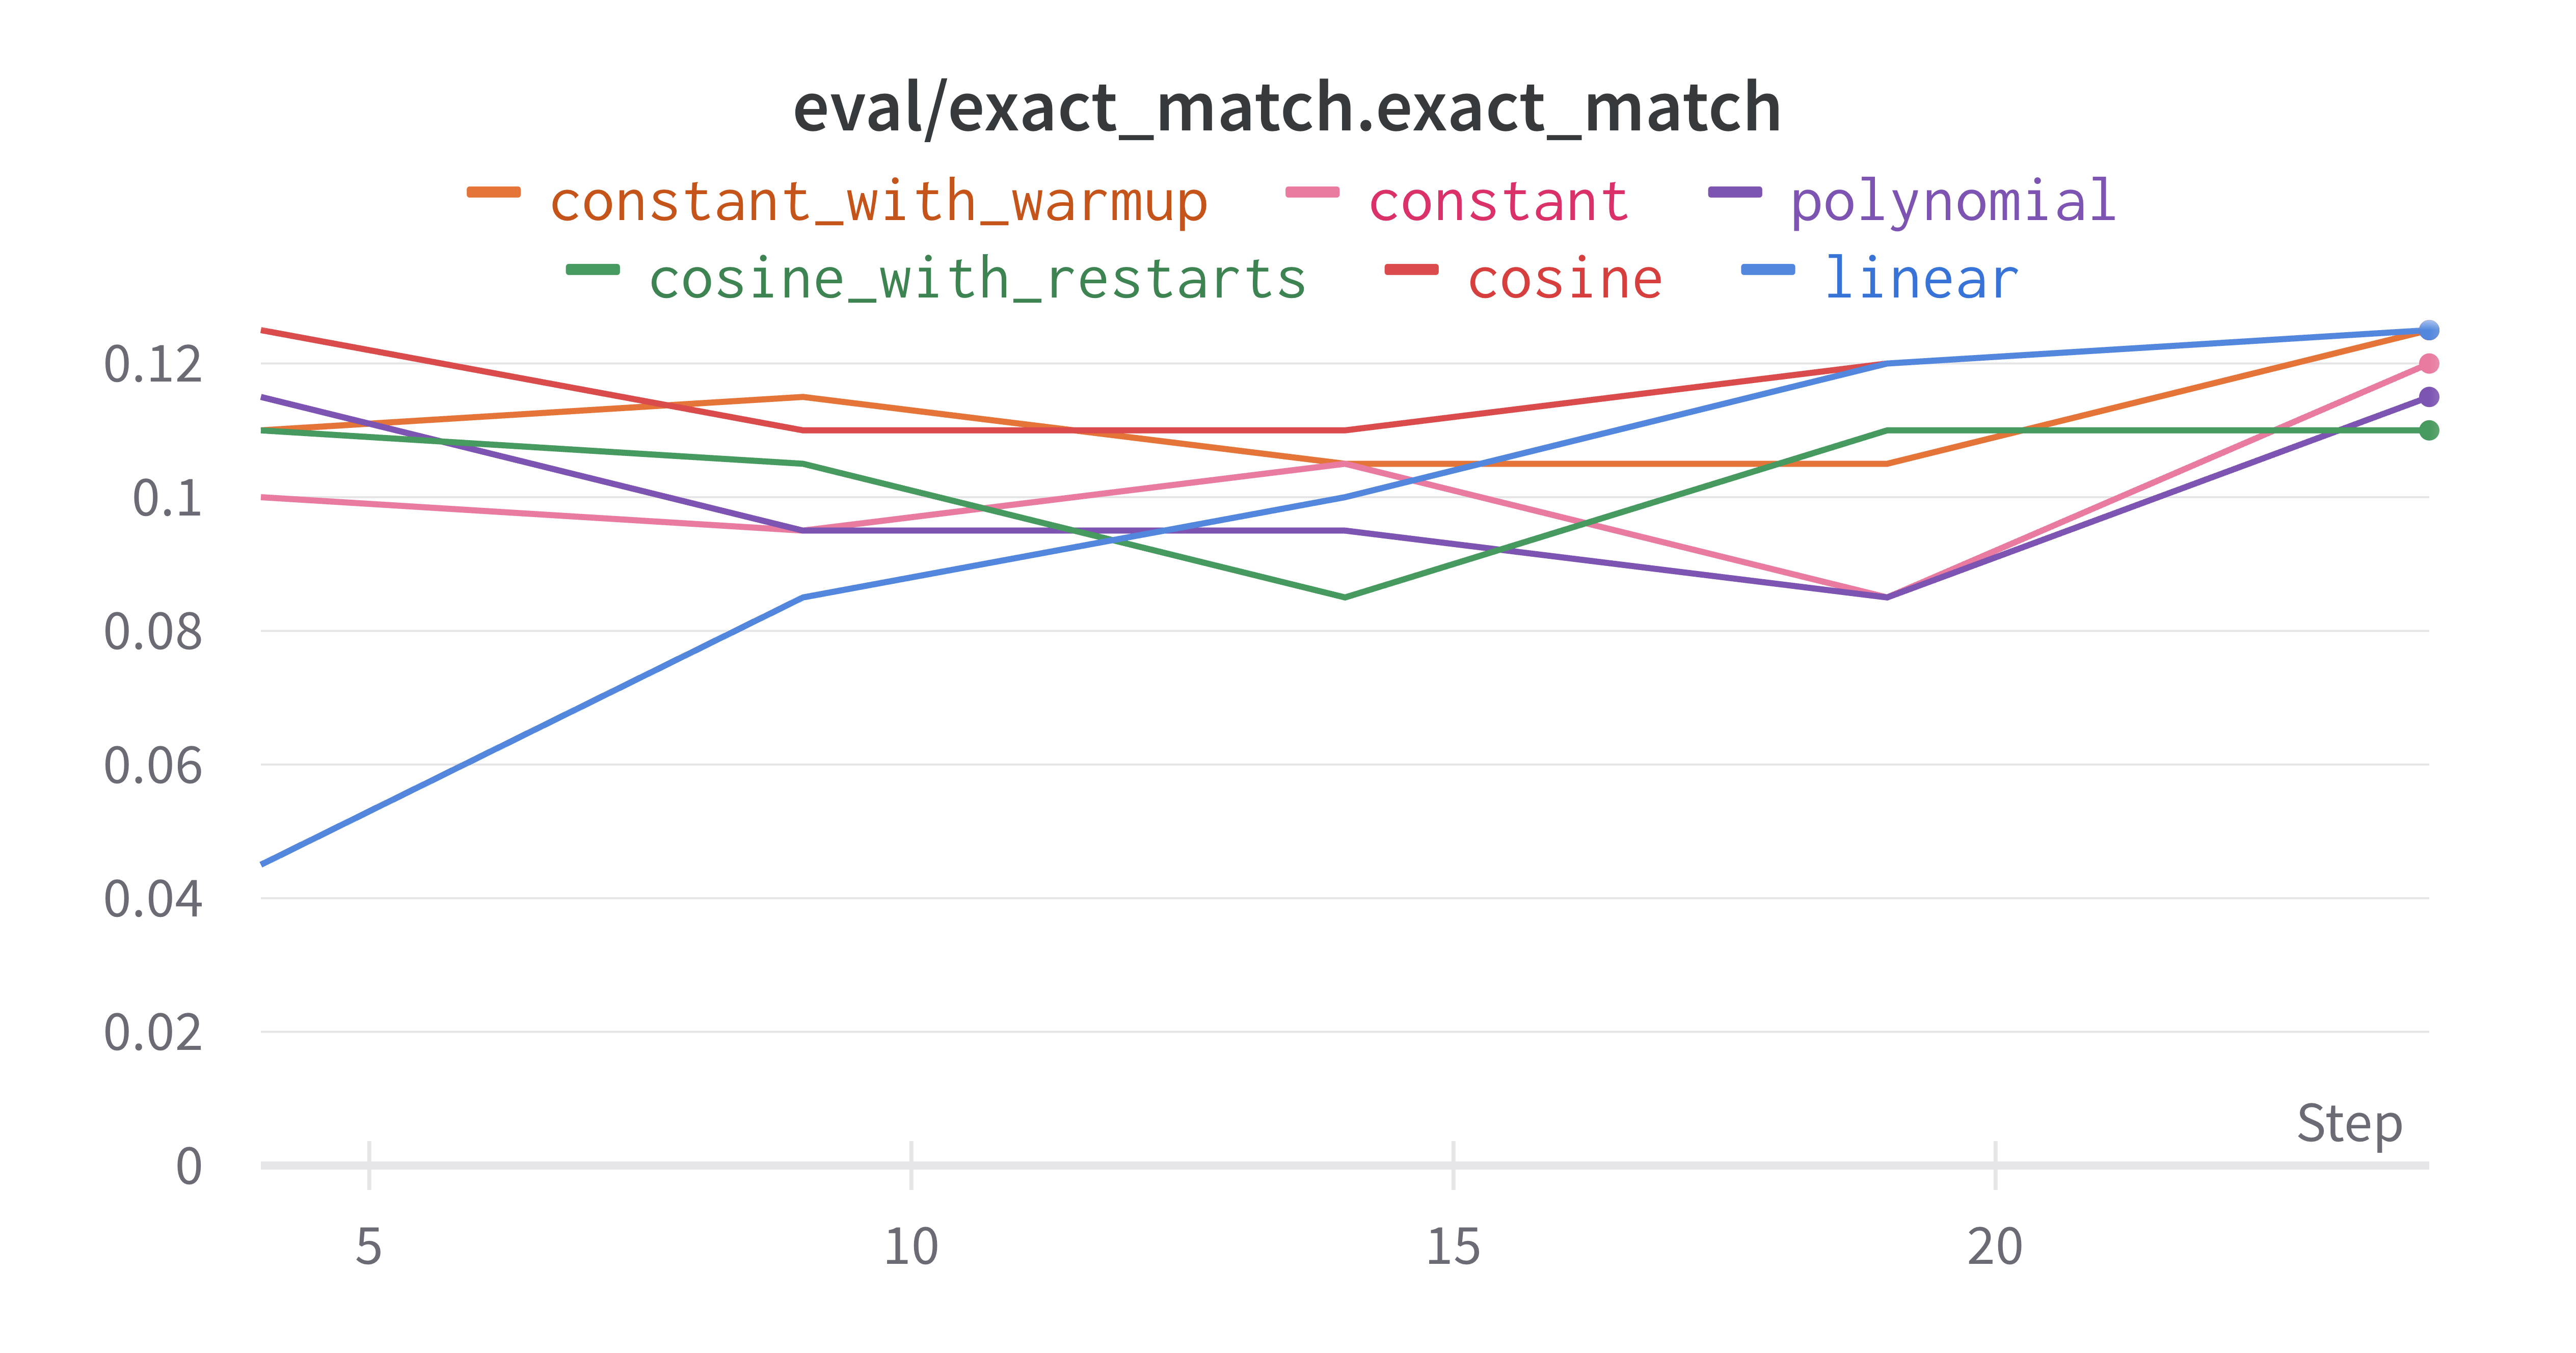
\includegraphics[width=.6\textwidth]{lr-s-em}
  \caption{Значение метрики Exact Match на валидационных данных}
  \label{lr-s-em}
\end{figure}

\begin{figure}[H]
  \centering
  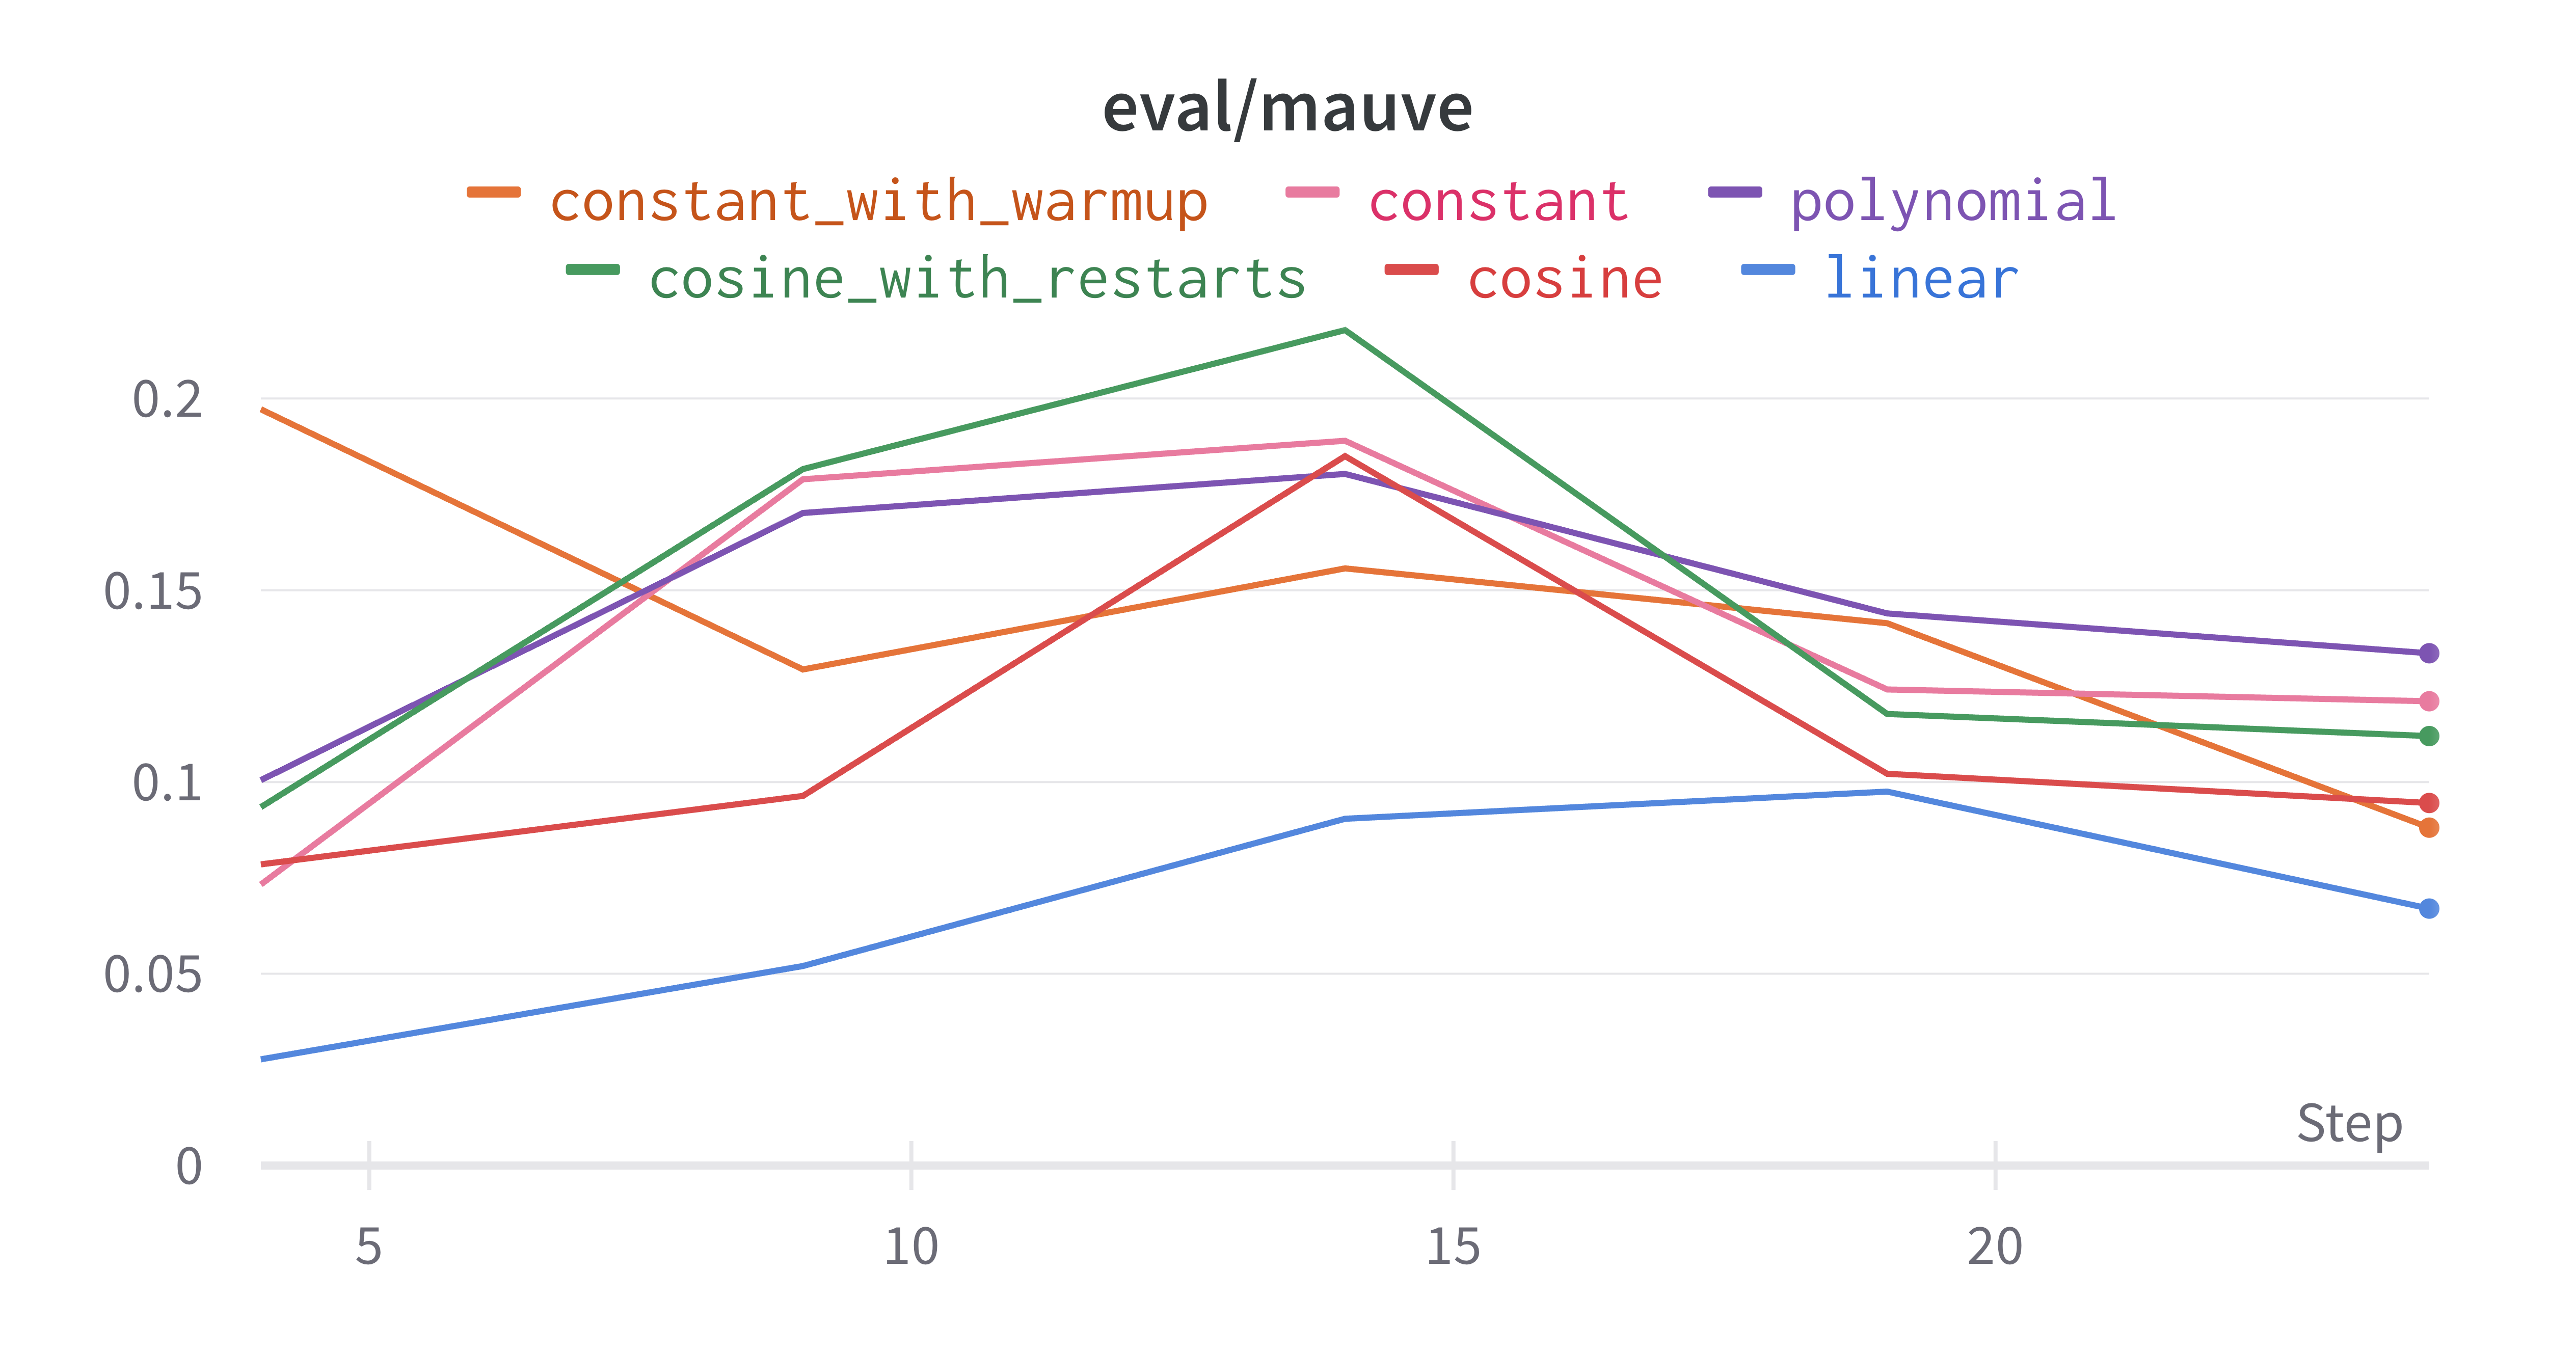
\includegraphics[width=.6\textwidth]{lr-s-mauve}
  \caption{Значение метрики MAUVE на валидационных данных}
  \label{lr-s-mauve}
\end{figure}

\begin{figure}[H]
  \centering
  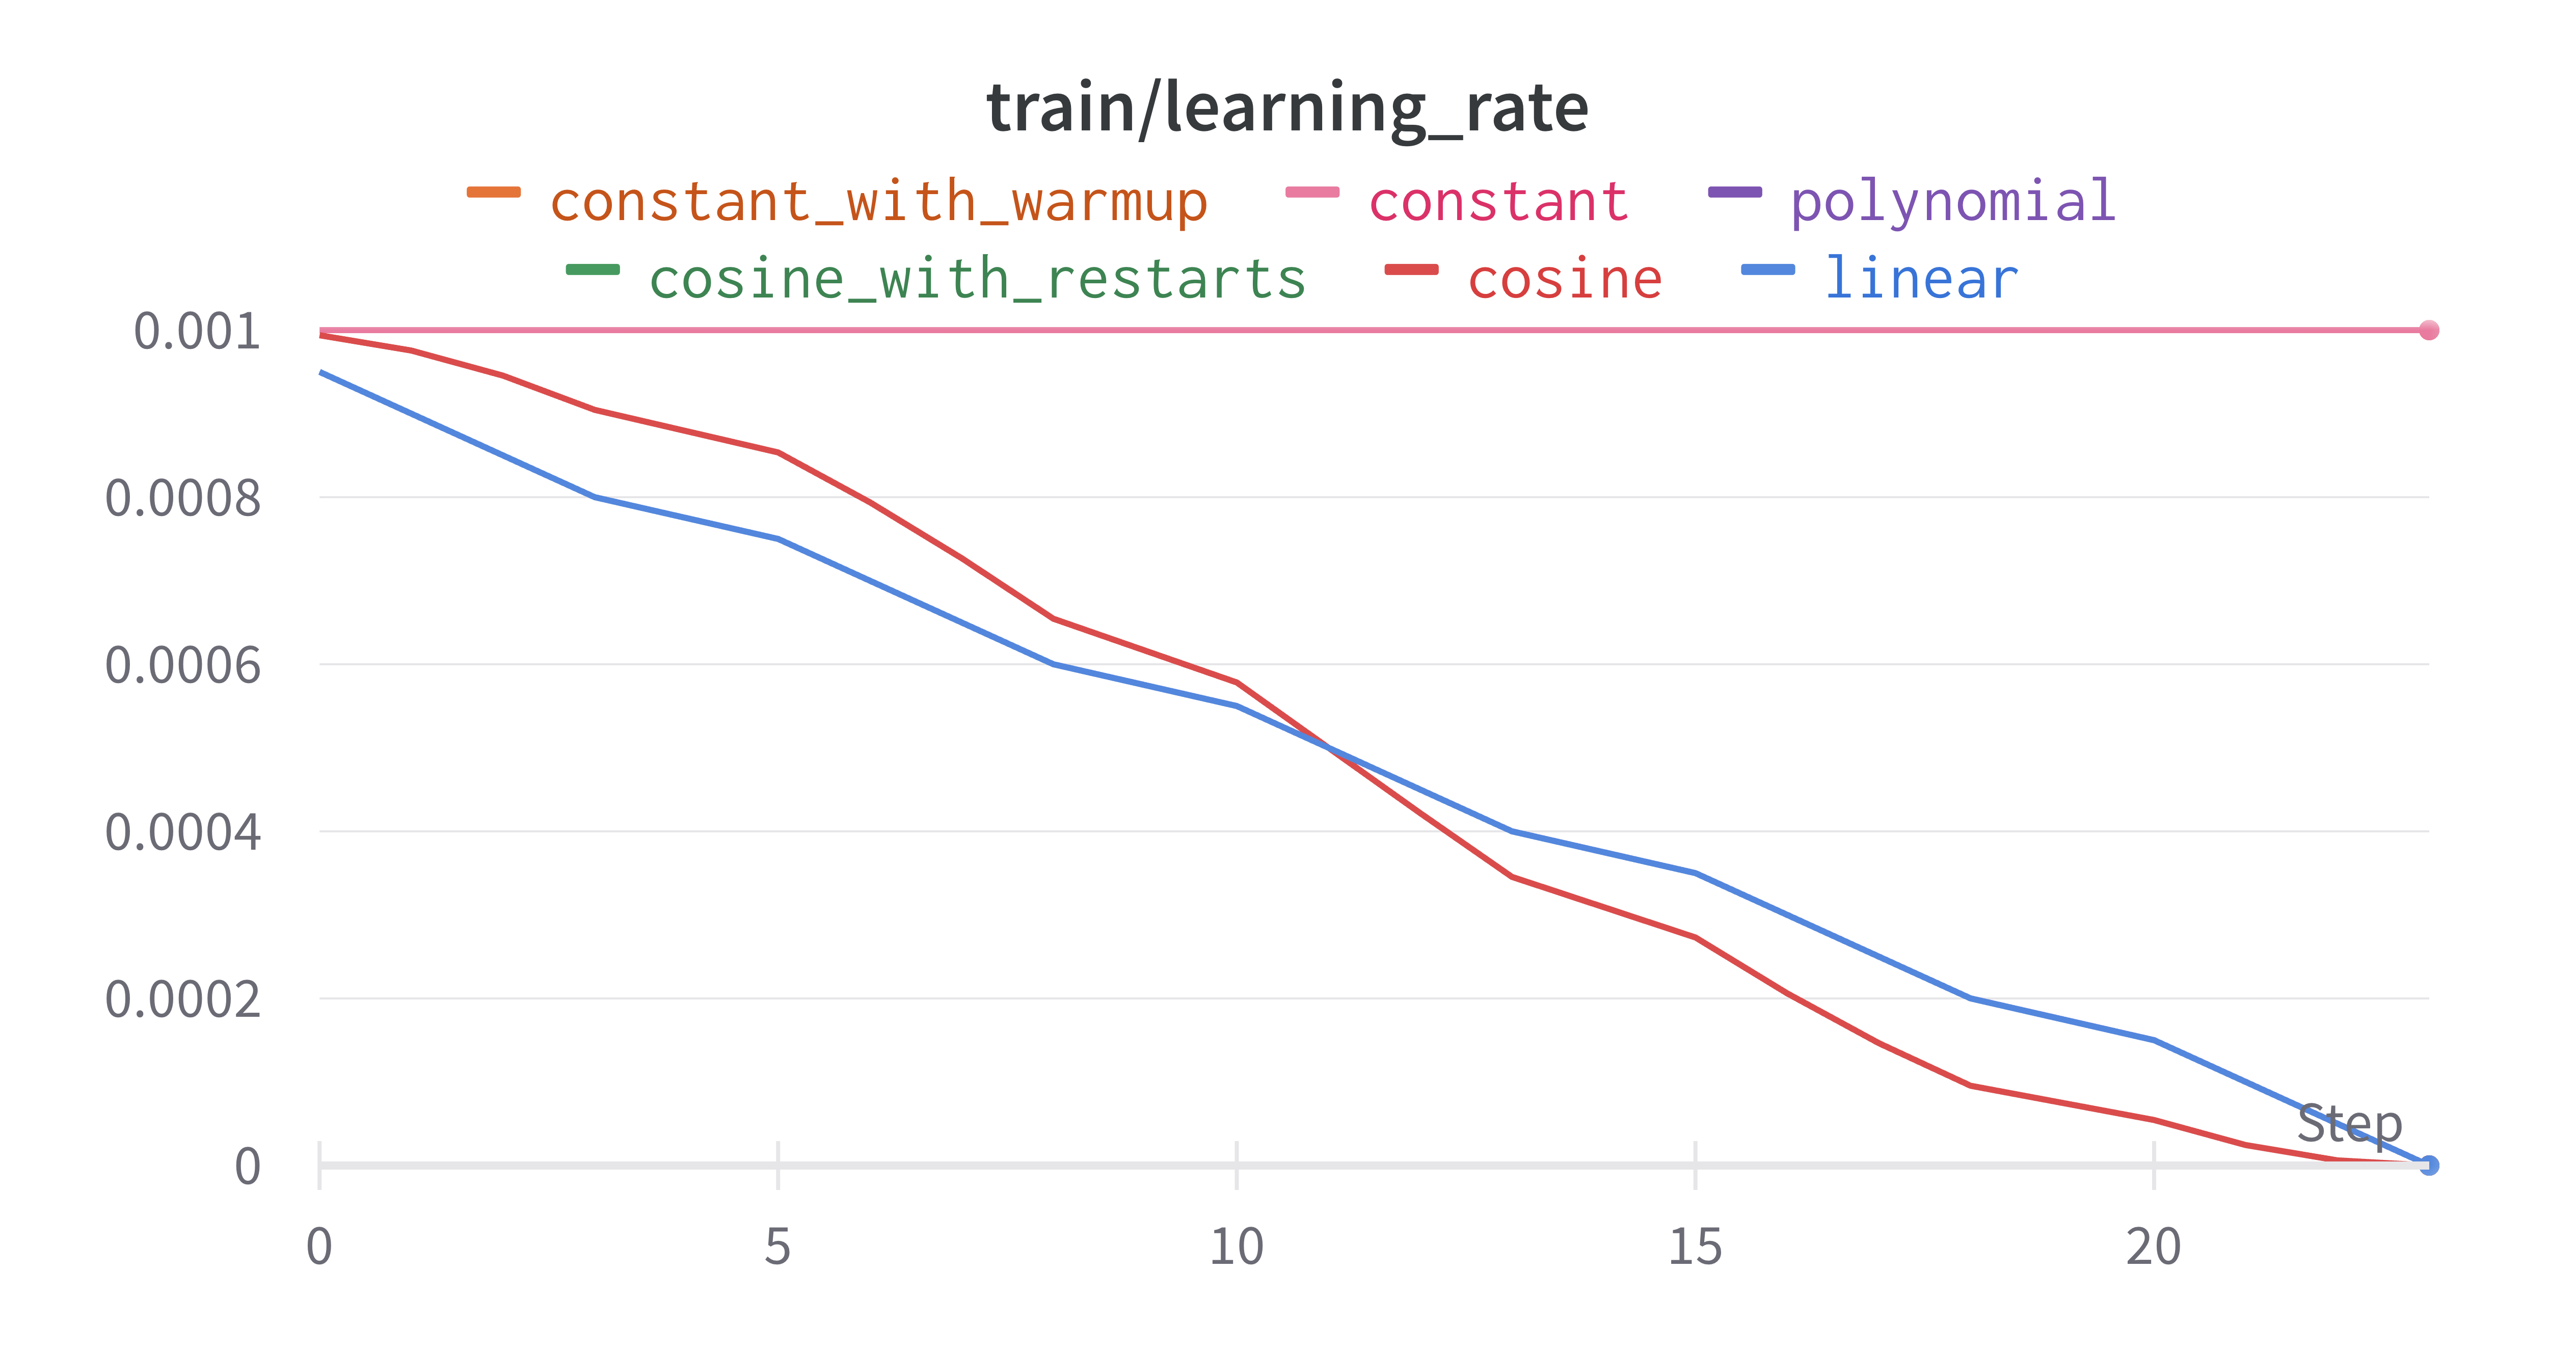
\includegraphics[width=.6\textwidth]{lr-s-lr}
  \caption{График изменения скорости обучения}
  \label{lr-s-lr}
\end{figure}

В следующих экспериментах при зафиксированном константном планировщике скорости обучения искалась наиболее эффективная скорость обучения. Стоит отметить, что при скорости обучения равной $1 \times 10^{-4}$ процесс обучения не завершился успешно. Из рисунков \ref{lr-train-loss}, \ref{lr-eval-loss}, \ref{lr-em}, \ref{lr-mauve} видно, что значения, близкие к $4 \times 10^{-4}$ и к $9 \times 10^{-4}$ показывают лучшие значения функций ошибок на всех выборках и лучшие значения метрик. Значение скорости обучения $9 \times 10^{-4}$ показывает результаты чуть лучше, чем $4 \times 10^{-4}$, быстрее достигая лучших значений. В целом, почти все значения скорости обучения показывают схожие результаты, но выбор оптимальных параметров для обучения на большей выборке может сказаться на качестве модели.

% LR
\begin{figure}[H]
  \centering
  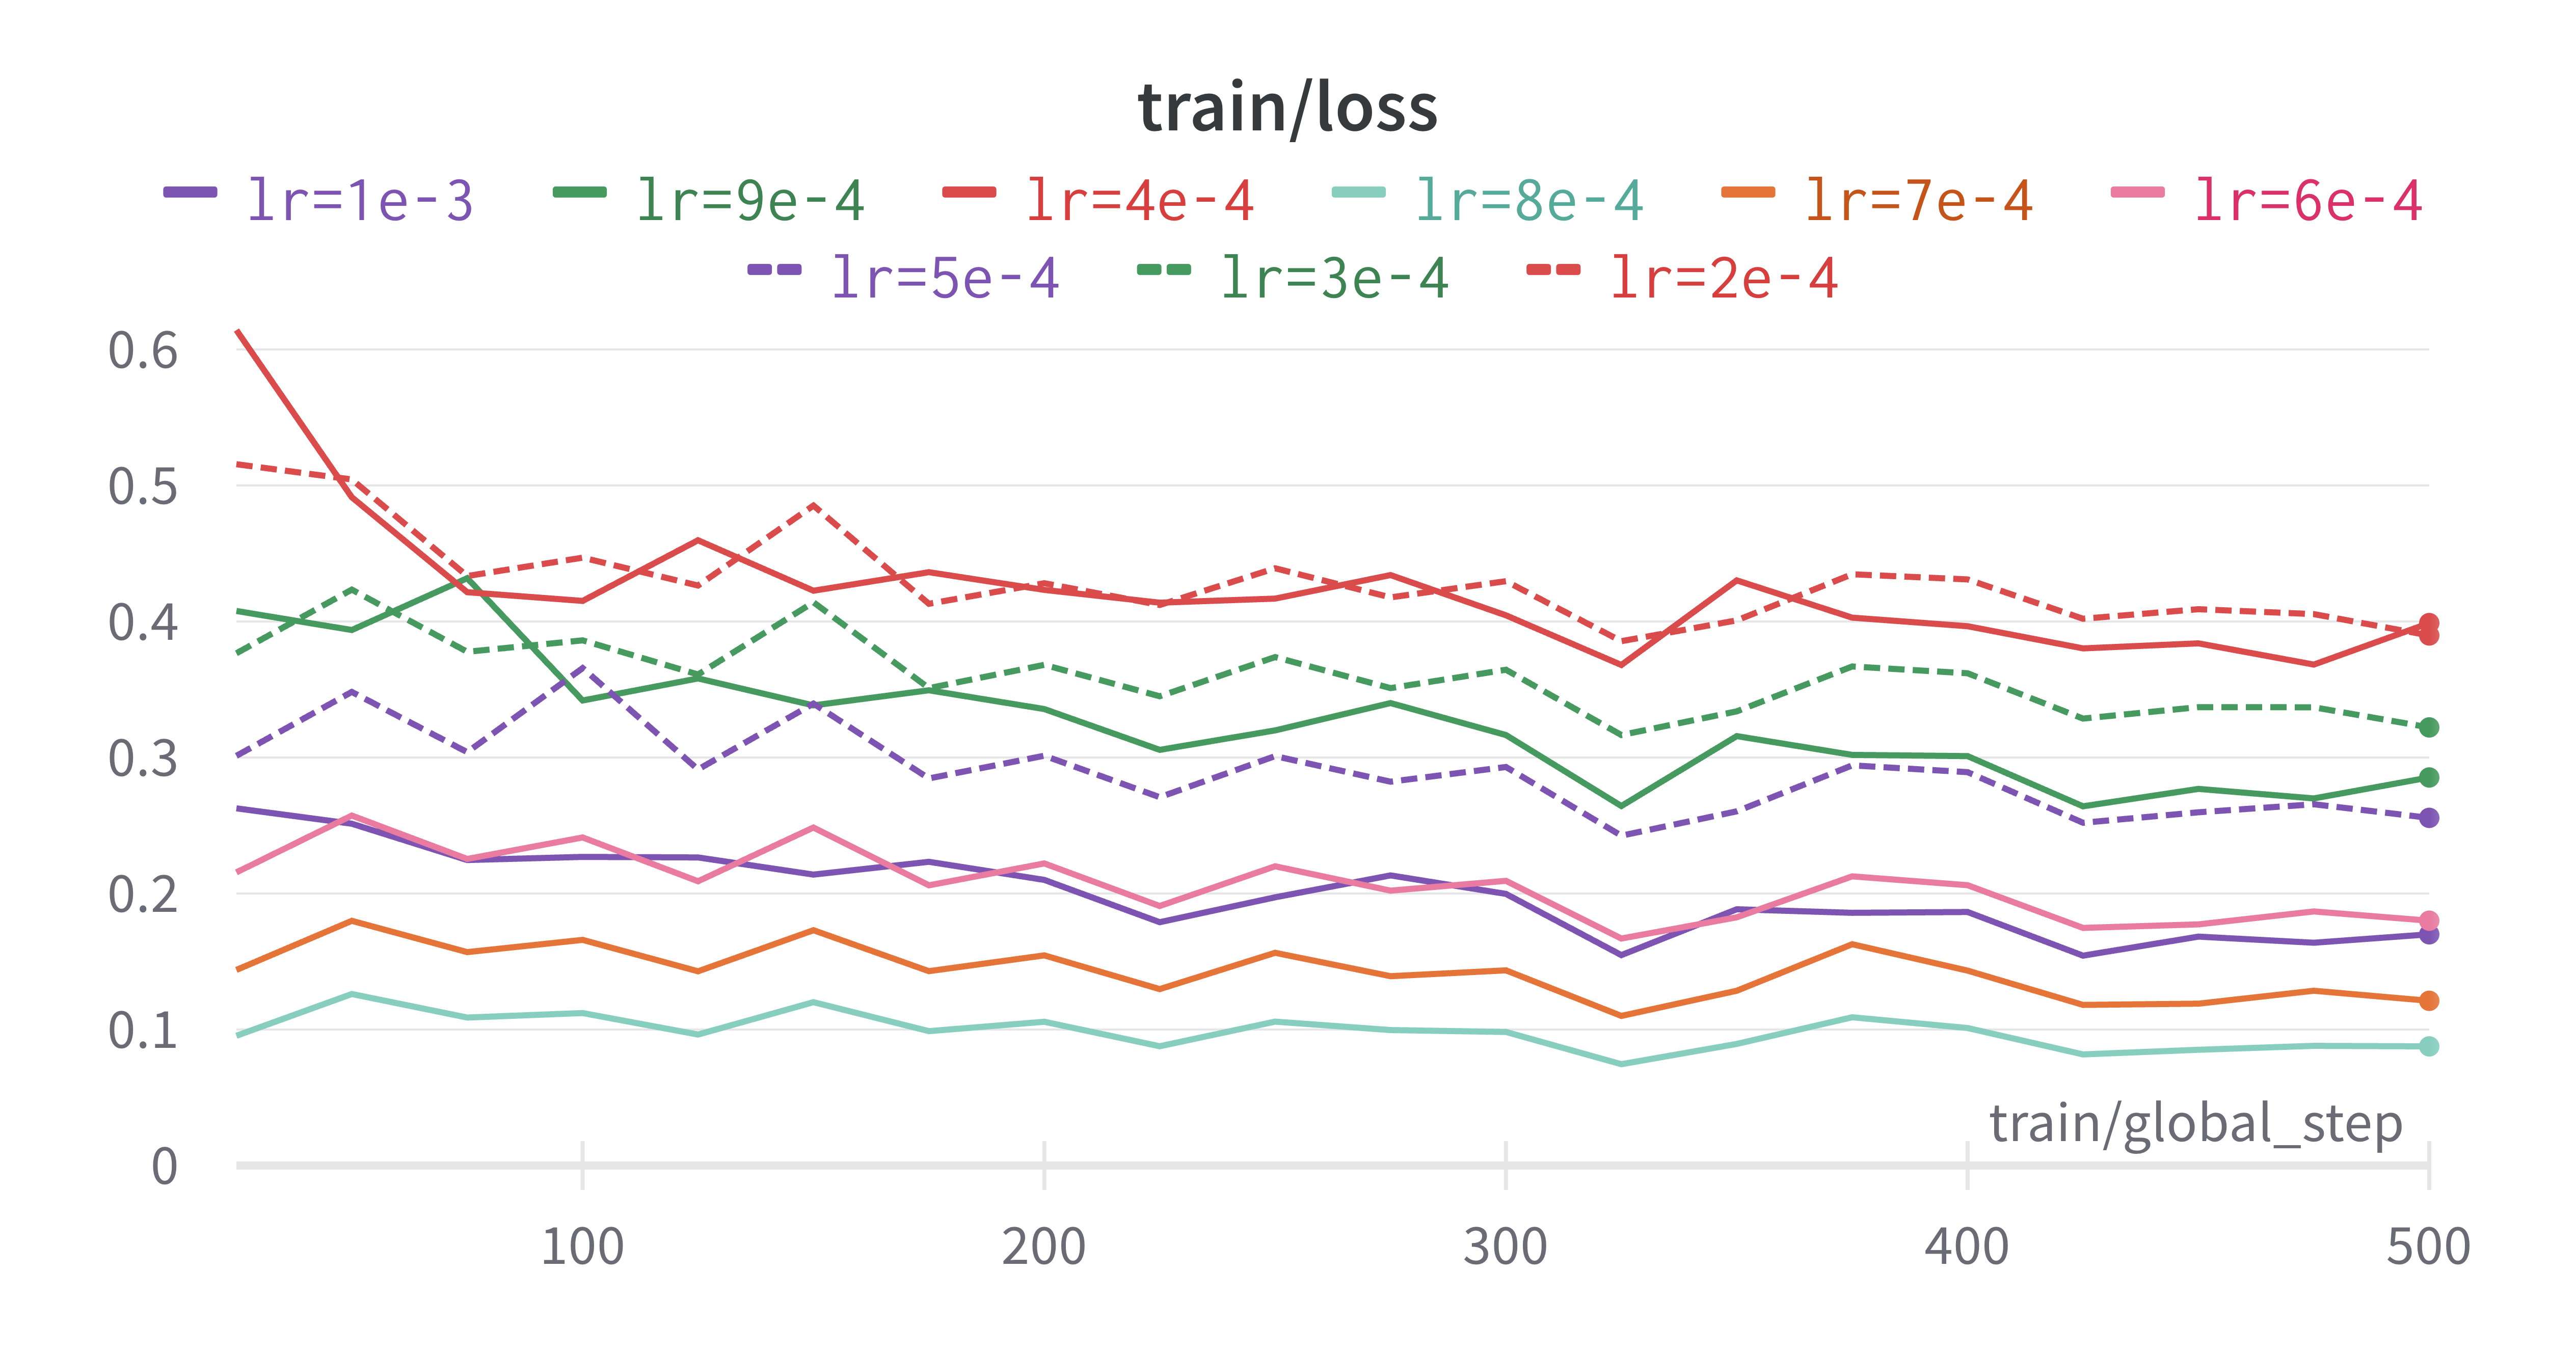
\includegraphics[width=.6\textwidth]{lr-train-loss}
  \caption{Значение функции ошибки на тренировочных данных}
  \label{lr-train-loss}
\end{figure}

\begin{figure}[H]
  \centering
  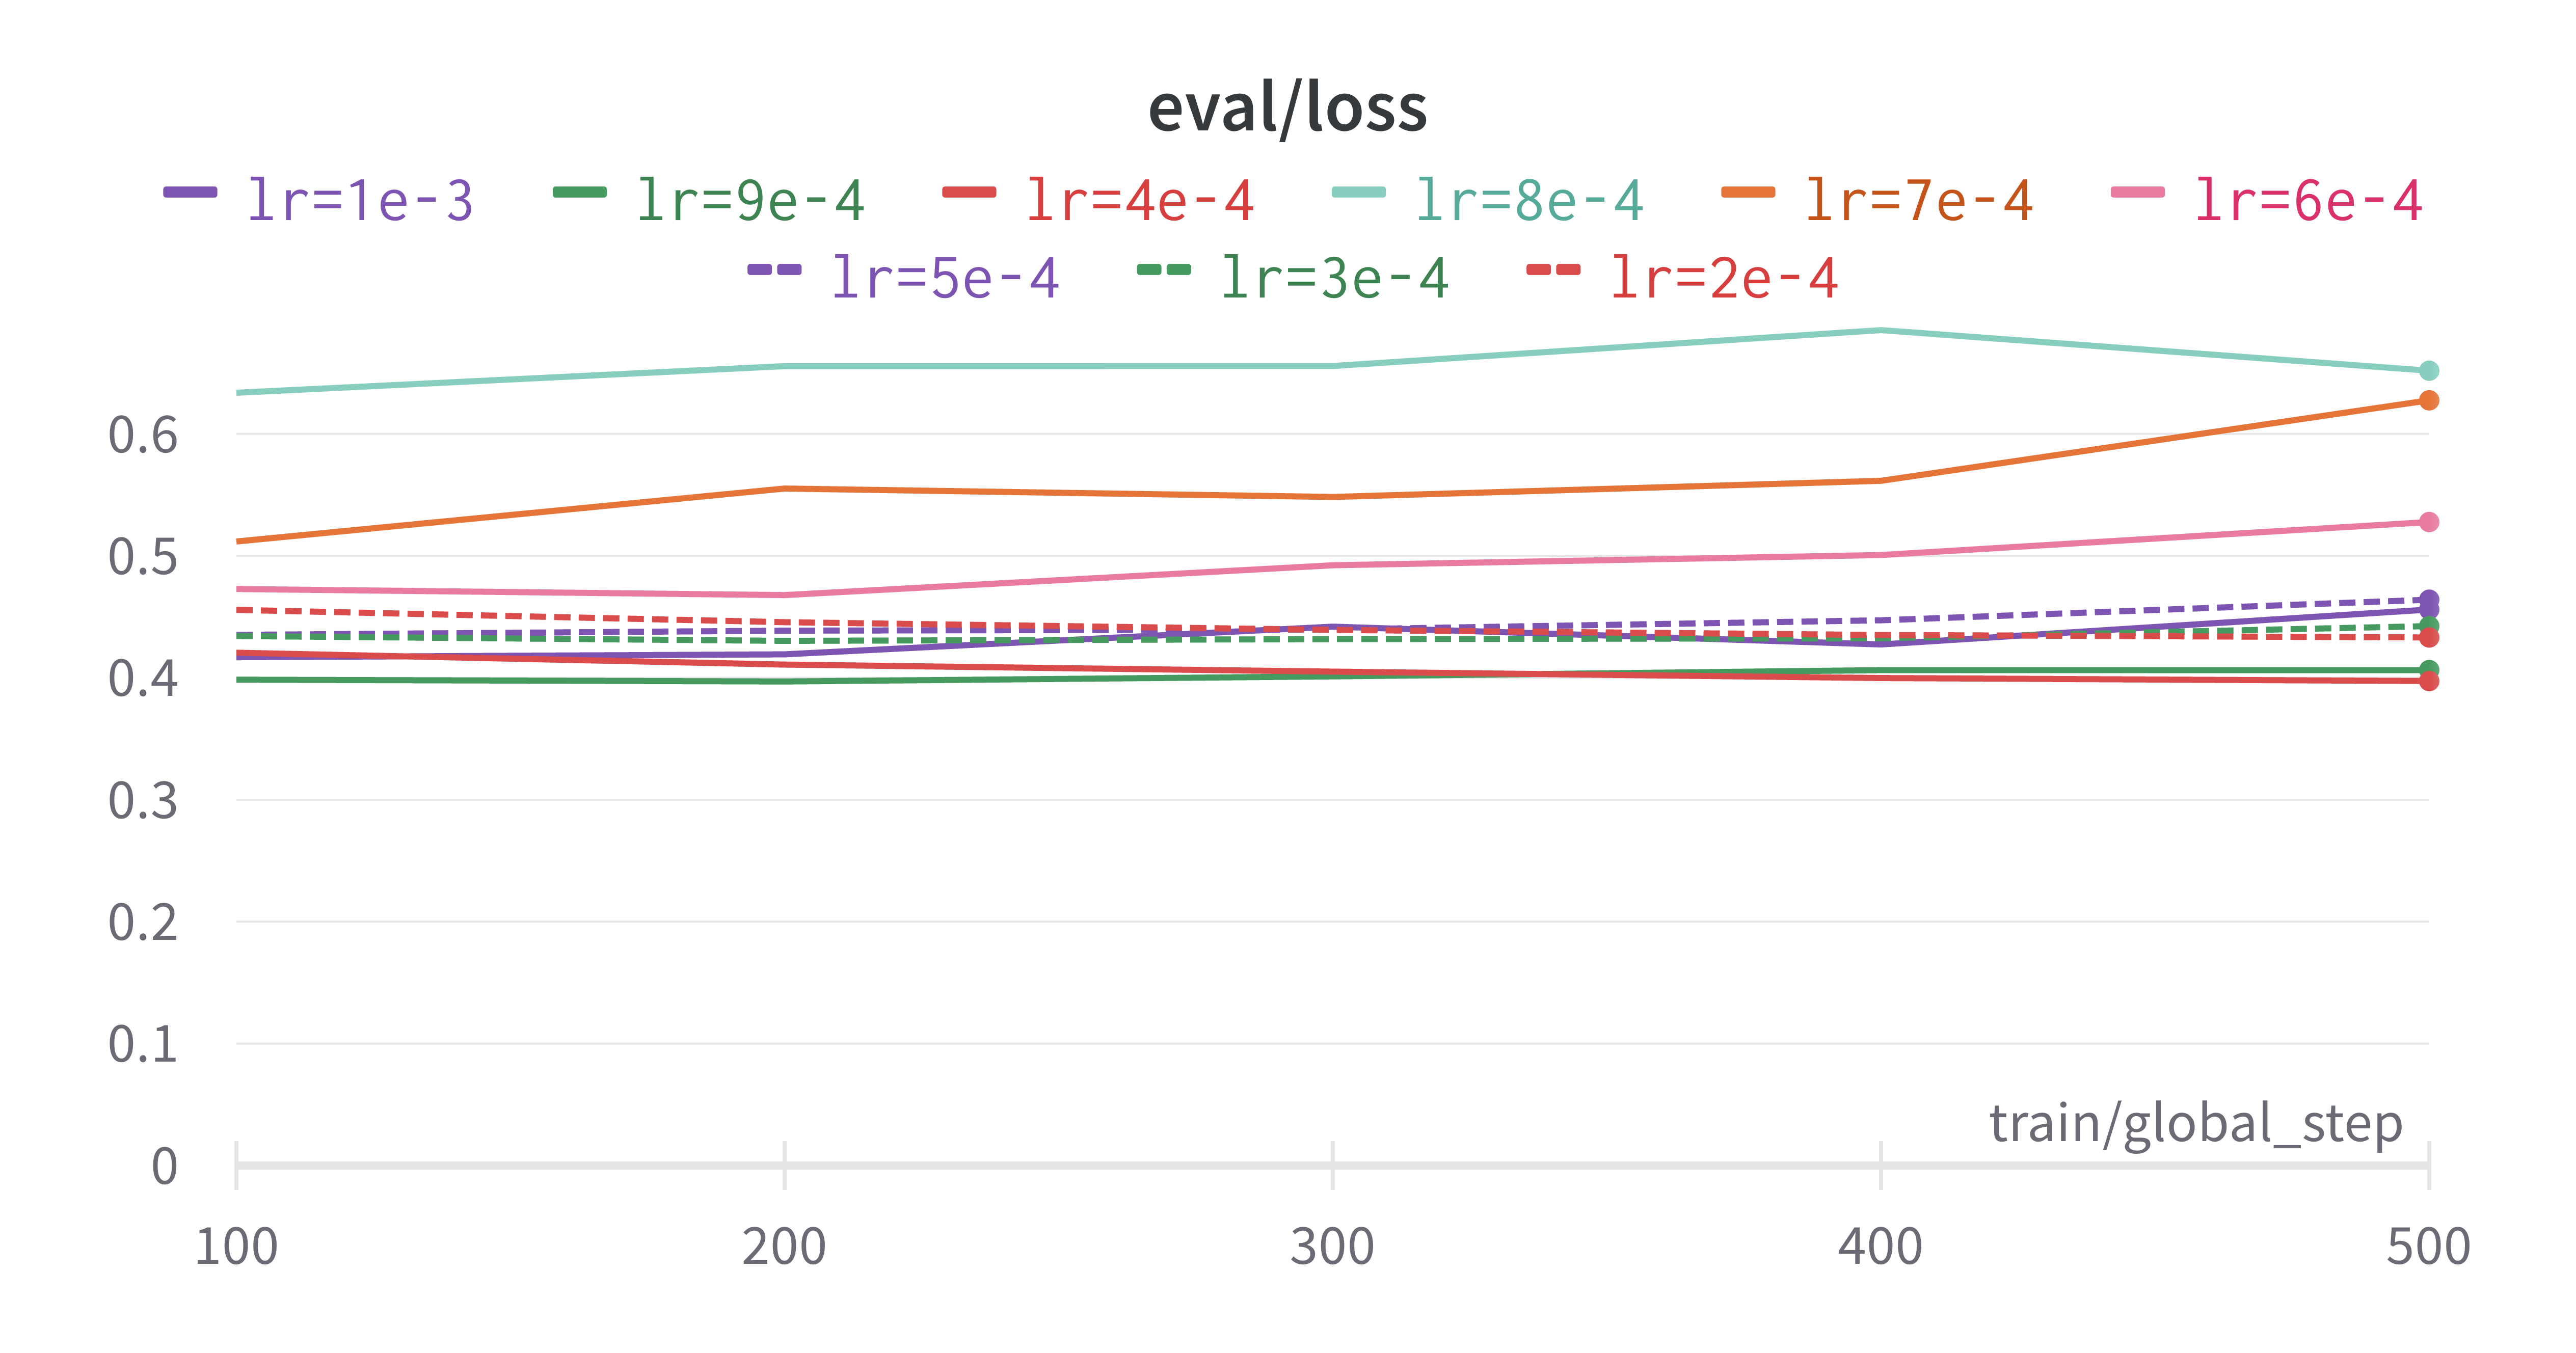
\includegraphics[width=.6\textwidth]{lr-eval-loss}
  \caption{Значение функции ошибки на валидационных данных}
  \label{lr-eval-loss}
\end{figure}

\begin{figure}[H]
  \centering
  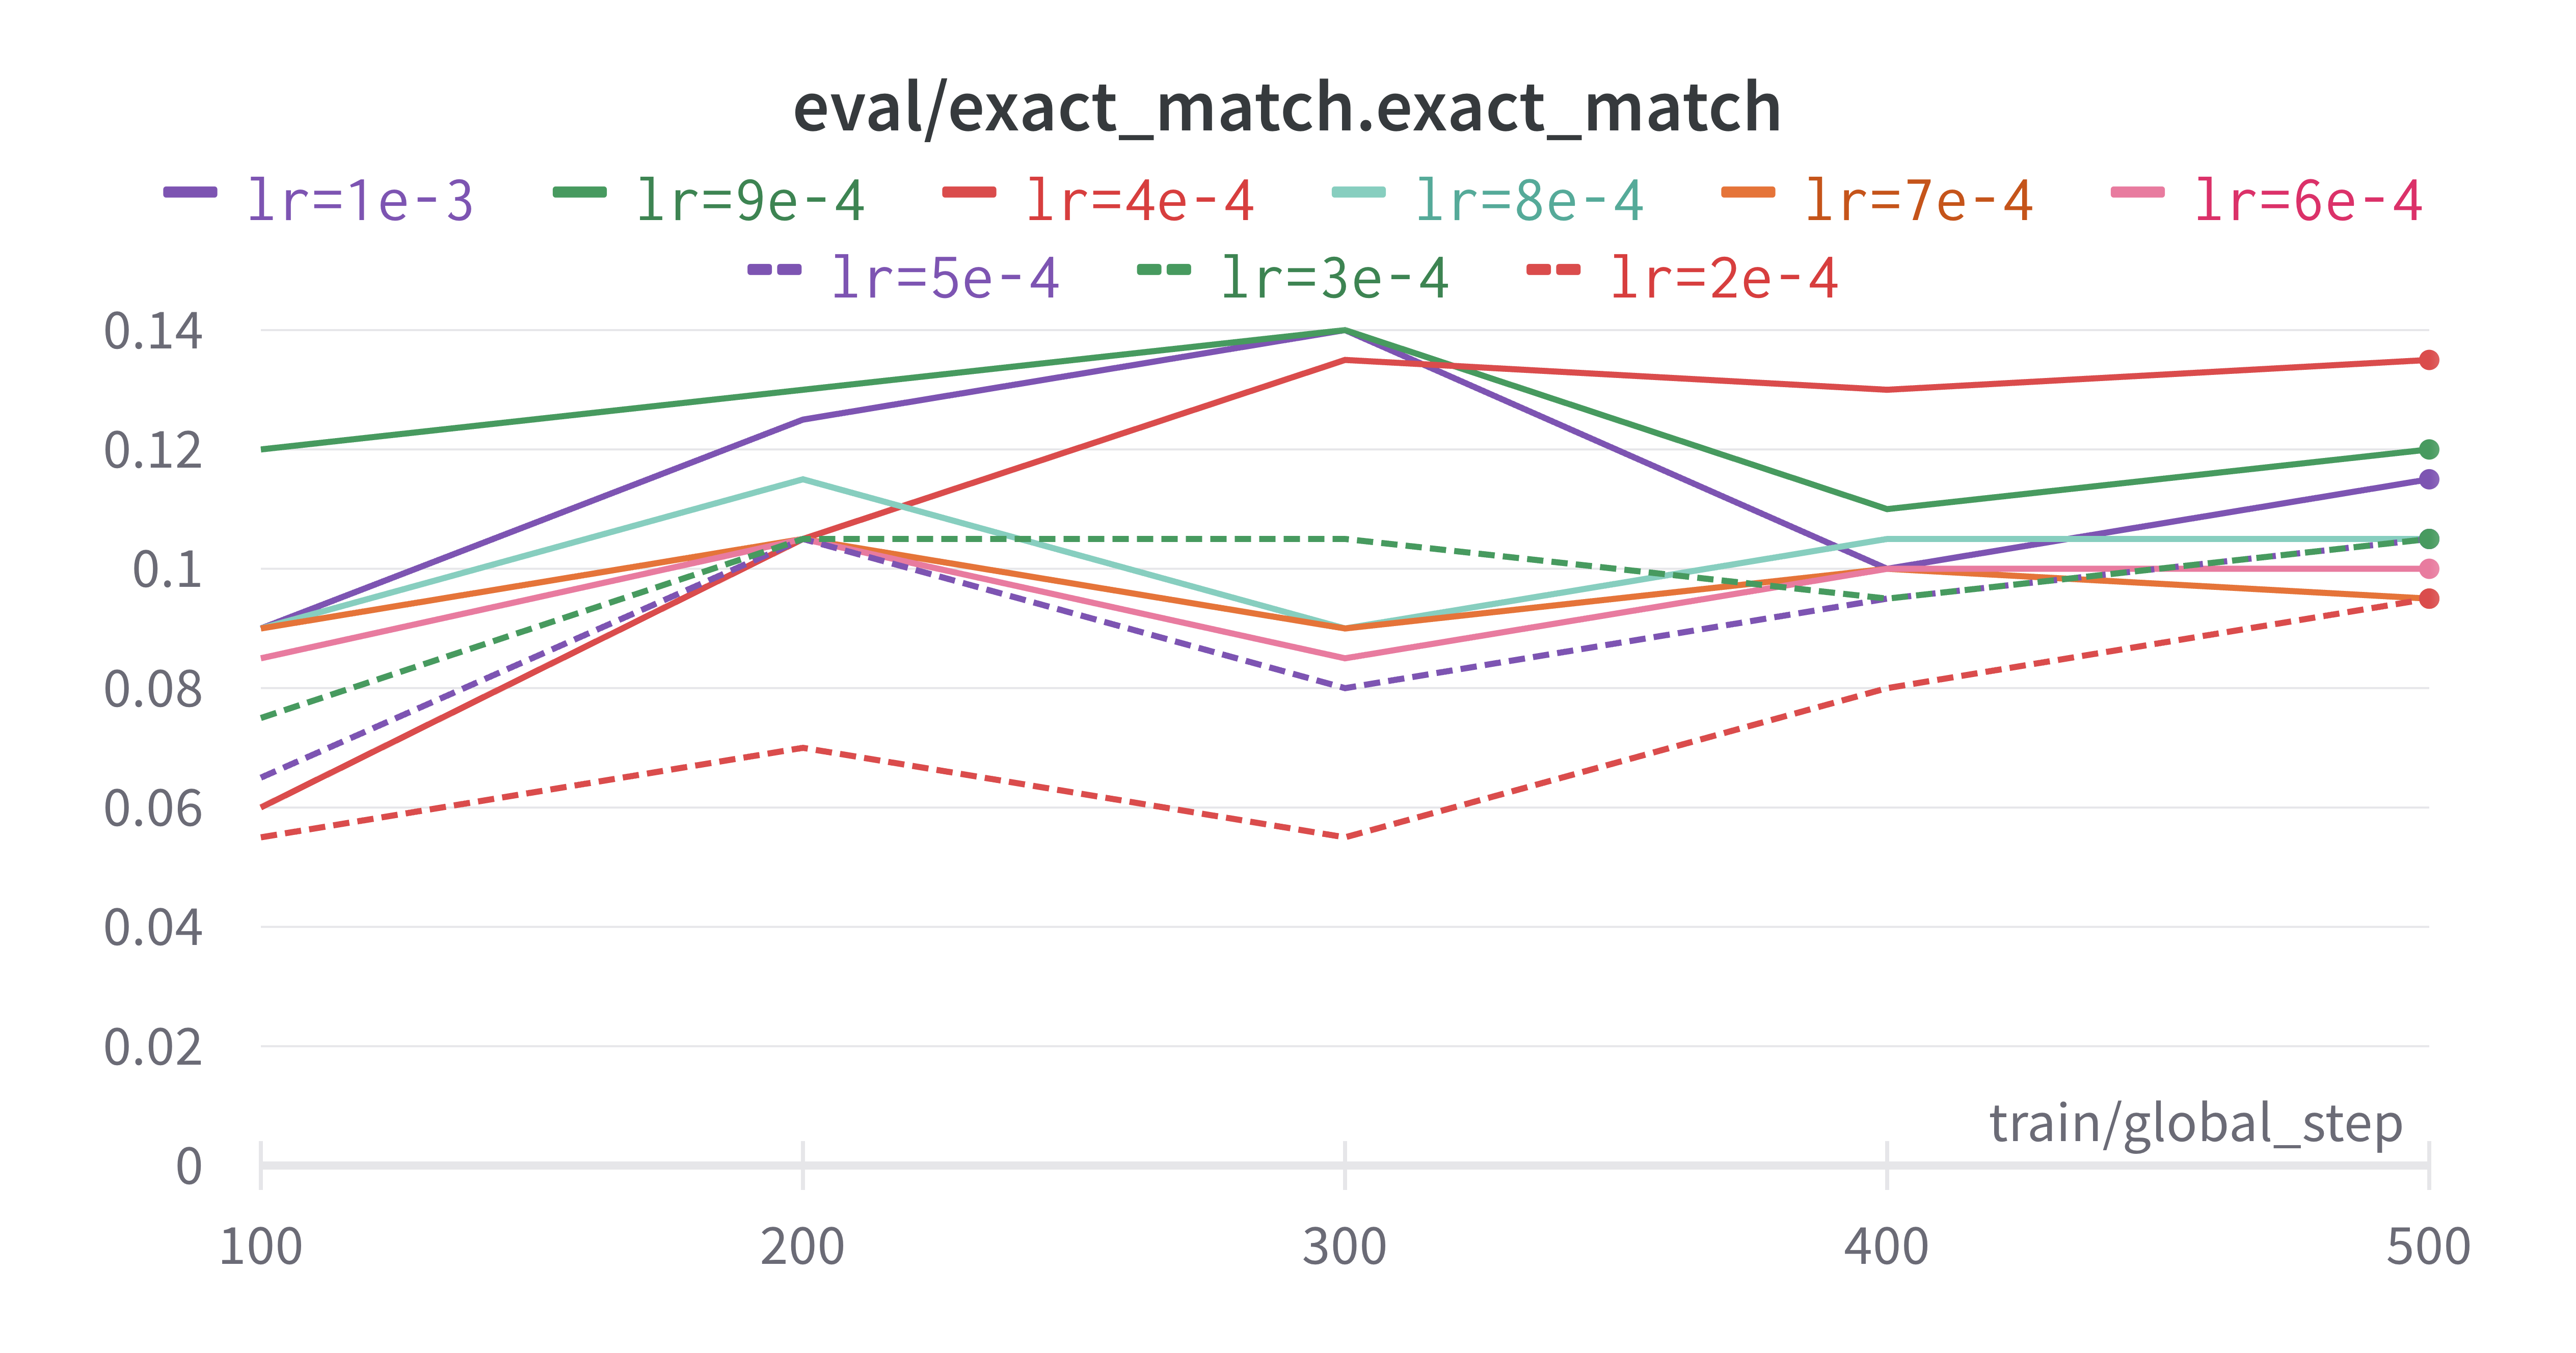
\includegraphics[width=.6\textwidth]{lr-em}
  \caption{Значение метрики Exact Match на валидационных данных}
  \label{lr-em}
\end{figure}

\begin{figure}[H]
  \centering
  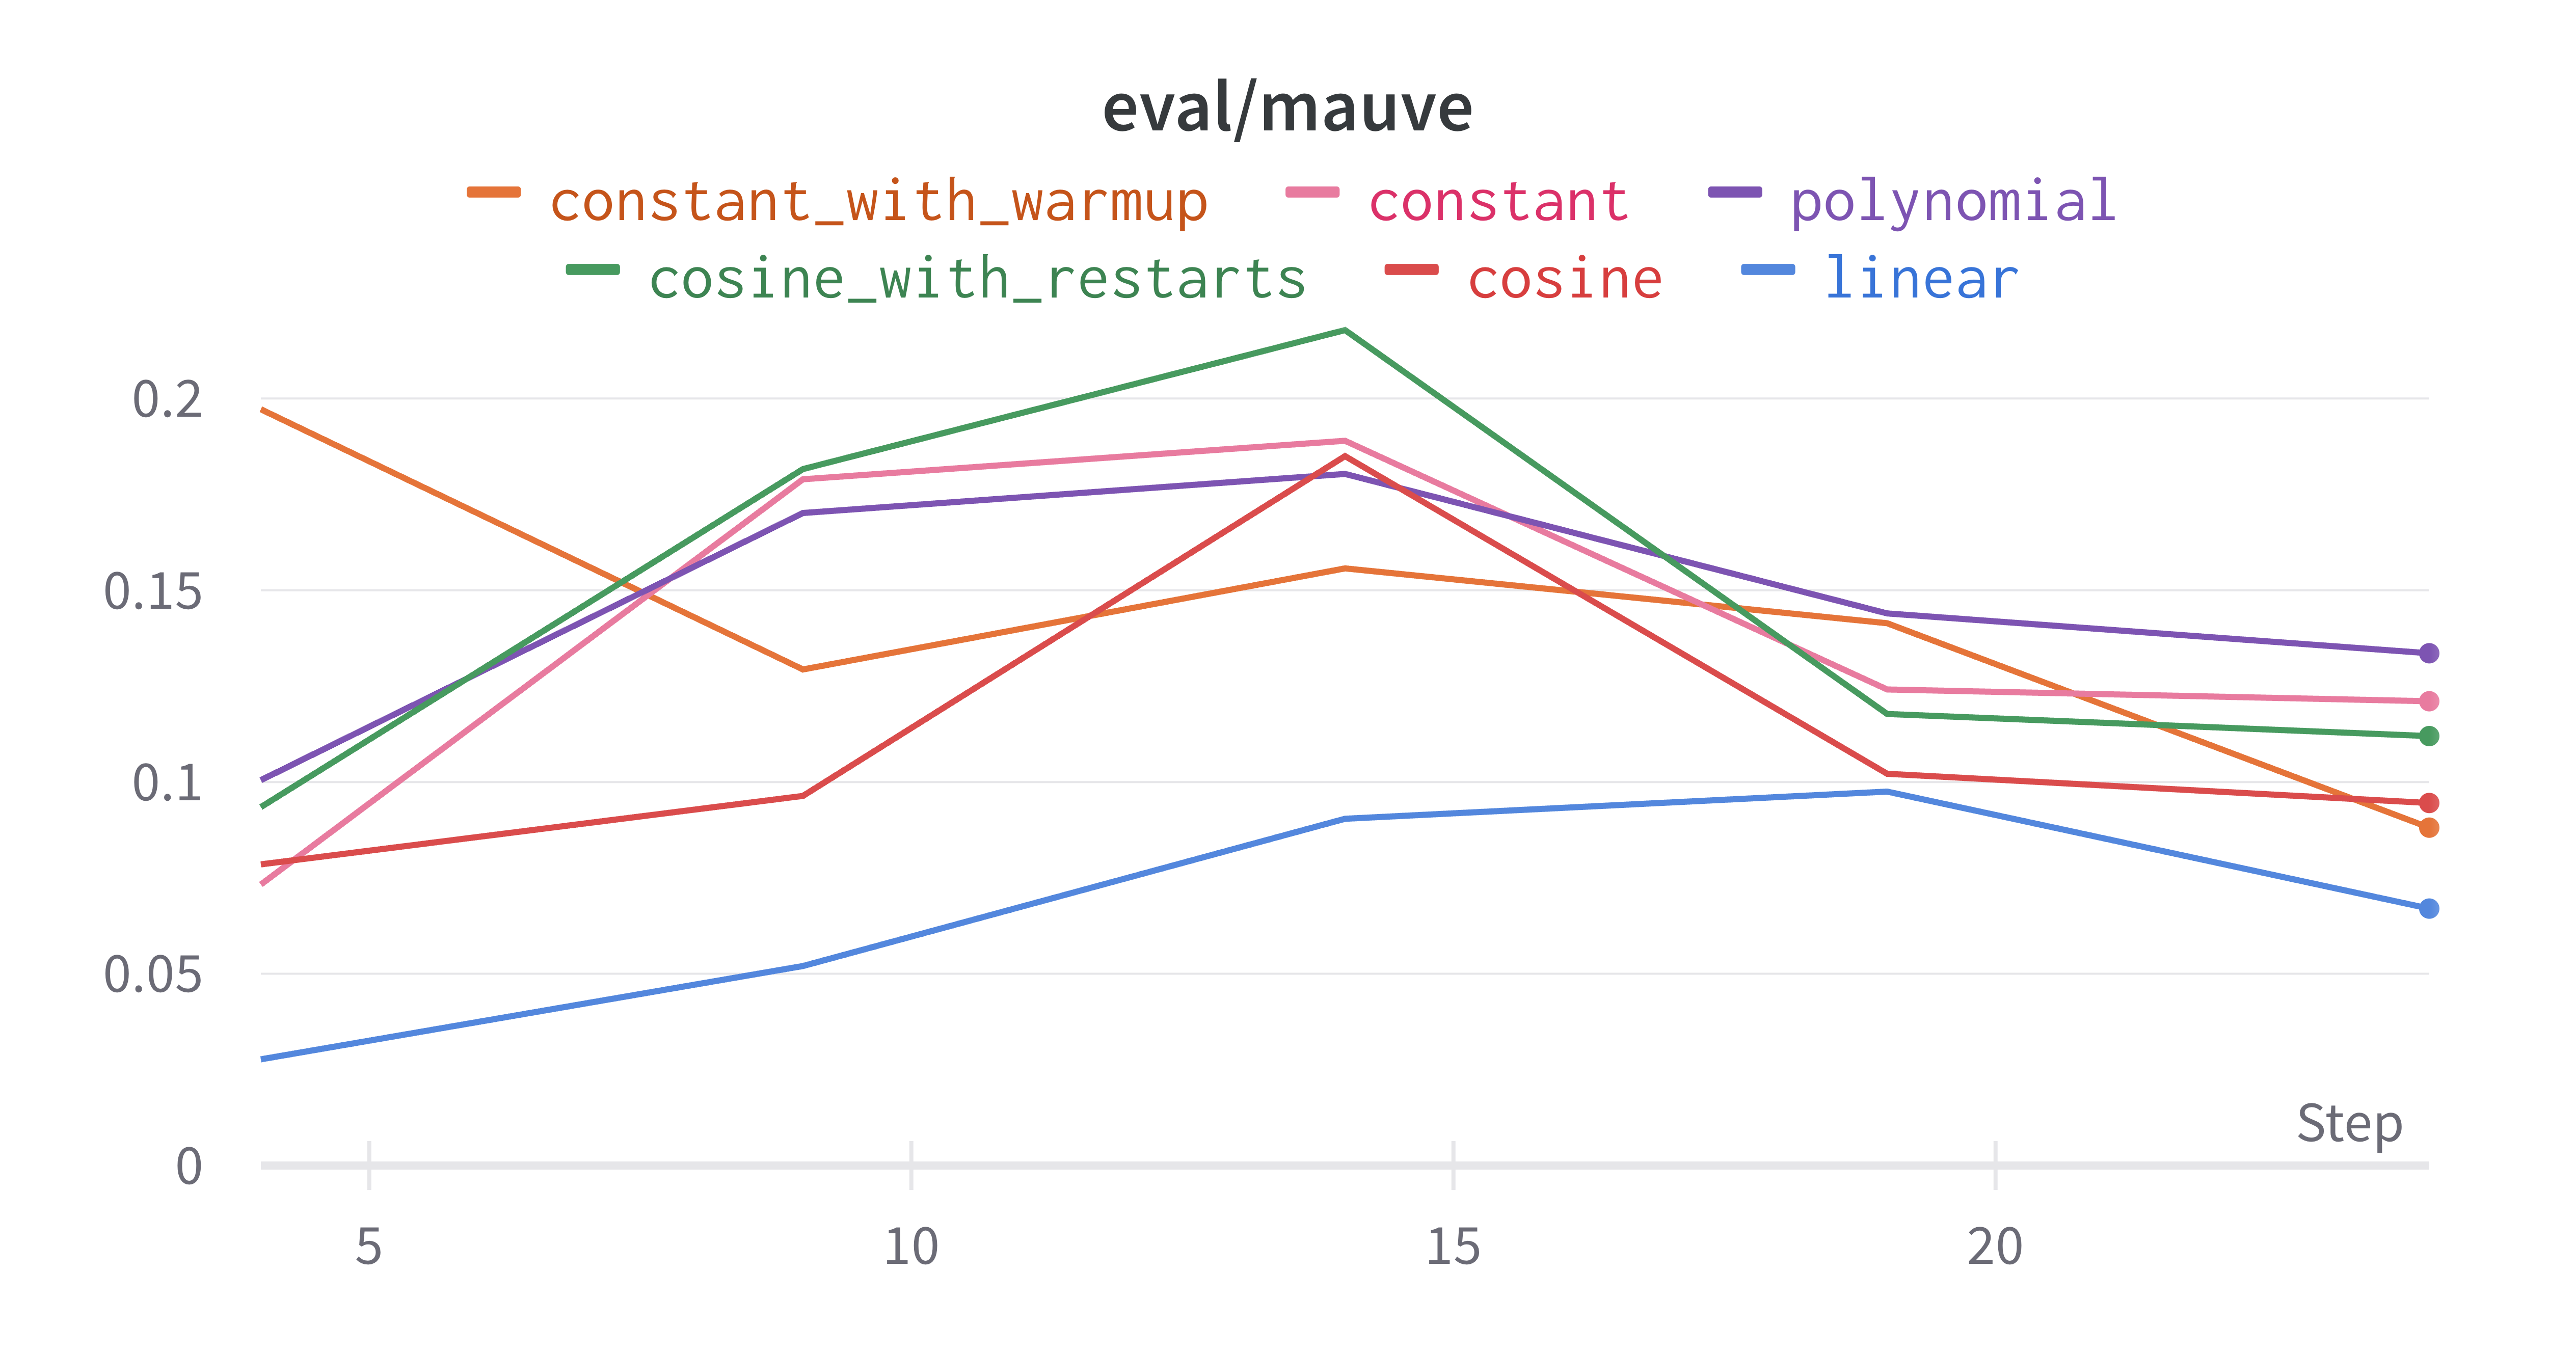
\includegraphics[width=.6\textwidth]{lr-s-mauve}
  \caption{Значение метрики MAUVE на валидационных данных}
  \label{lr-mauve}
\end{figure}

Исходя из всех экспериментов можно сделать вывод, что оптимальные параметры для обучения будут константный планировщик скорости обучения и скорость обучения со значением $9 \times 10^{-4}$

\section{ОБУЧЕНИЕ ИТОГОВОЙ МОДЕЛИ}

С подобранными ранее параметрами на была обучена итоговая модель. Общее количество операций, произведенных во время обучения, составило $2 \times 10^{18}$. Количество токенов, которые фигурировали в процессе обучения -- $25 \times 10^{6}$. Процесс обучения виден на рисунках \ref{total-train-loss}, \ref{total-eval-loss}, \ref{total-em}, \ref{total-mauve}. Низкие значения метрик Exact Match и MAUVE можно объяснить сложностью поставленной модели задачи: в диалогах часто ответы формируются исходя из внешних условий, в которых производился диалог с неигровым персонажем, которые сложно получить из данных игры в формате естественного языка. Метрика Exact Match довольно грубо оценивает результат генерации -- переформулированная фраза в такой оценке даст значение 0. Тем не менее, такую систему получилось обучить на потребительском оборудовании на неплохие результаты. Далее идет пример диалога, который был произведен с моделью.

\texttt{\\Below is the definition of in-game NPC.\\
  The Mad Lord\\
  Alignment: Chaotic Neutral\\
  Description: A mysterious figure who resides in a castle called Caste Maluradek in the middle of a forest. He is a powerful wizard who has the ability to manipulate the elements and create illusions.\\
  Personality traits: He is obsessed with power and will stop at nothing to achieve his goals.\\
  Flaws: He wants to prove that he is the most powerful wizard in the world.
  Motivation: The Mad Lord is a mysterious figure who is driven by his desire for power. He is a master manipulator and will use any means necessary to achieve his goals. He is a powerful wizard who is not afraid to use his magic to get what he wants. He is also a bit of a showman, as he enjoys creating elaborate illusions to impress his guests.\\
  Dialogue history:\\
  Player: START DIALOGUE\\
  NPC: Salutations to the travelers. Welcome to Castle Maluradek. I am your adversary.\\
  Player query: Does the adversary have a name?\\
  Respond to player's query based on defined NPC:\\
  ANSWER: I do not have a name. I am a practitioner of magic. I work in the fields of the great forest.}

Больше примеров можно увидеть в приложении \ref{app:diagogue}.

\begin{figure}[H]
  \centering
  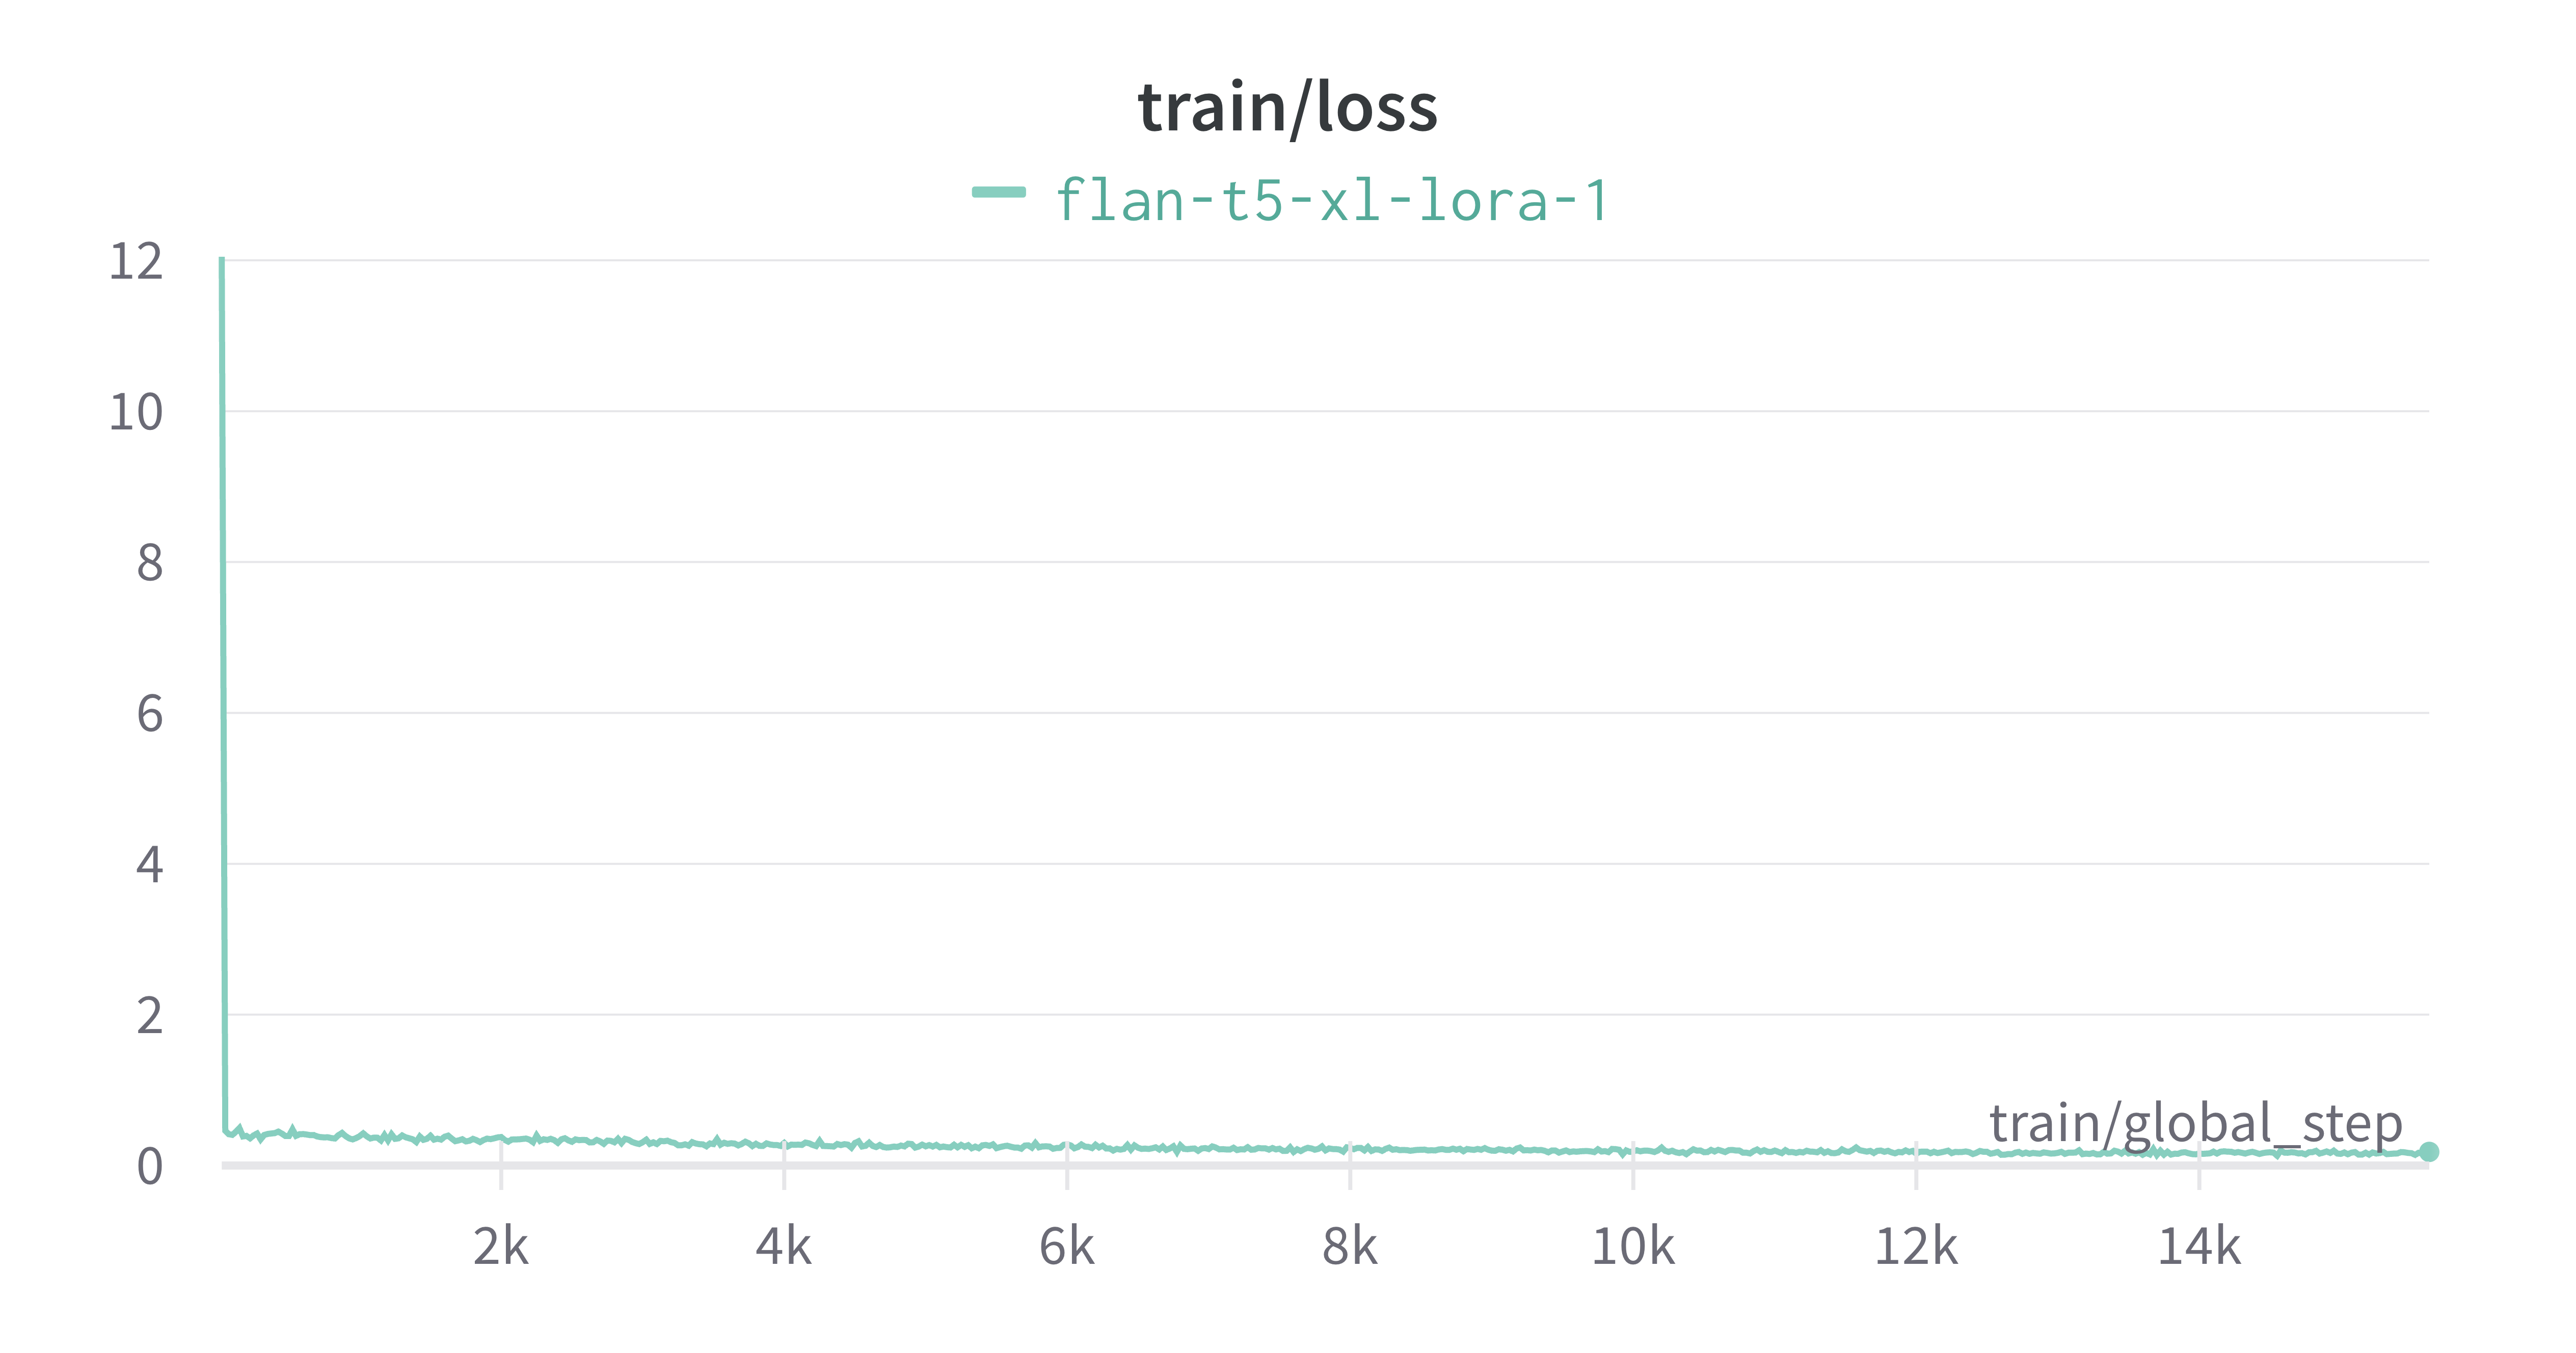
\includegraphics[width=.6\textwidth]{total-train-loss}
  \caption{Значение функции ошибки на тренировочных данных}
  \label{total-train-loss}
\end{figure}

\begin{figure}[H]
  \centering
  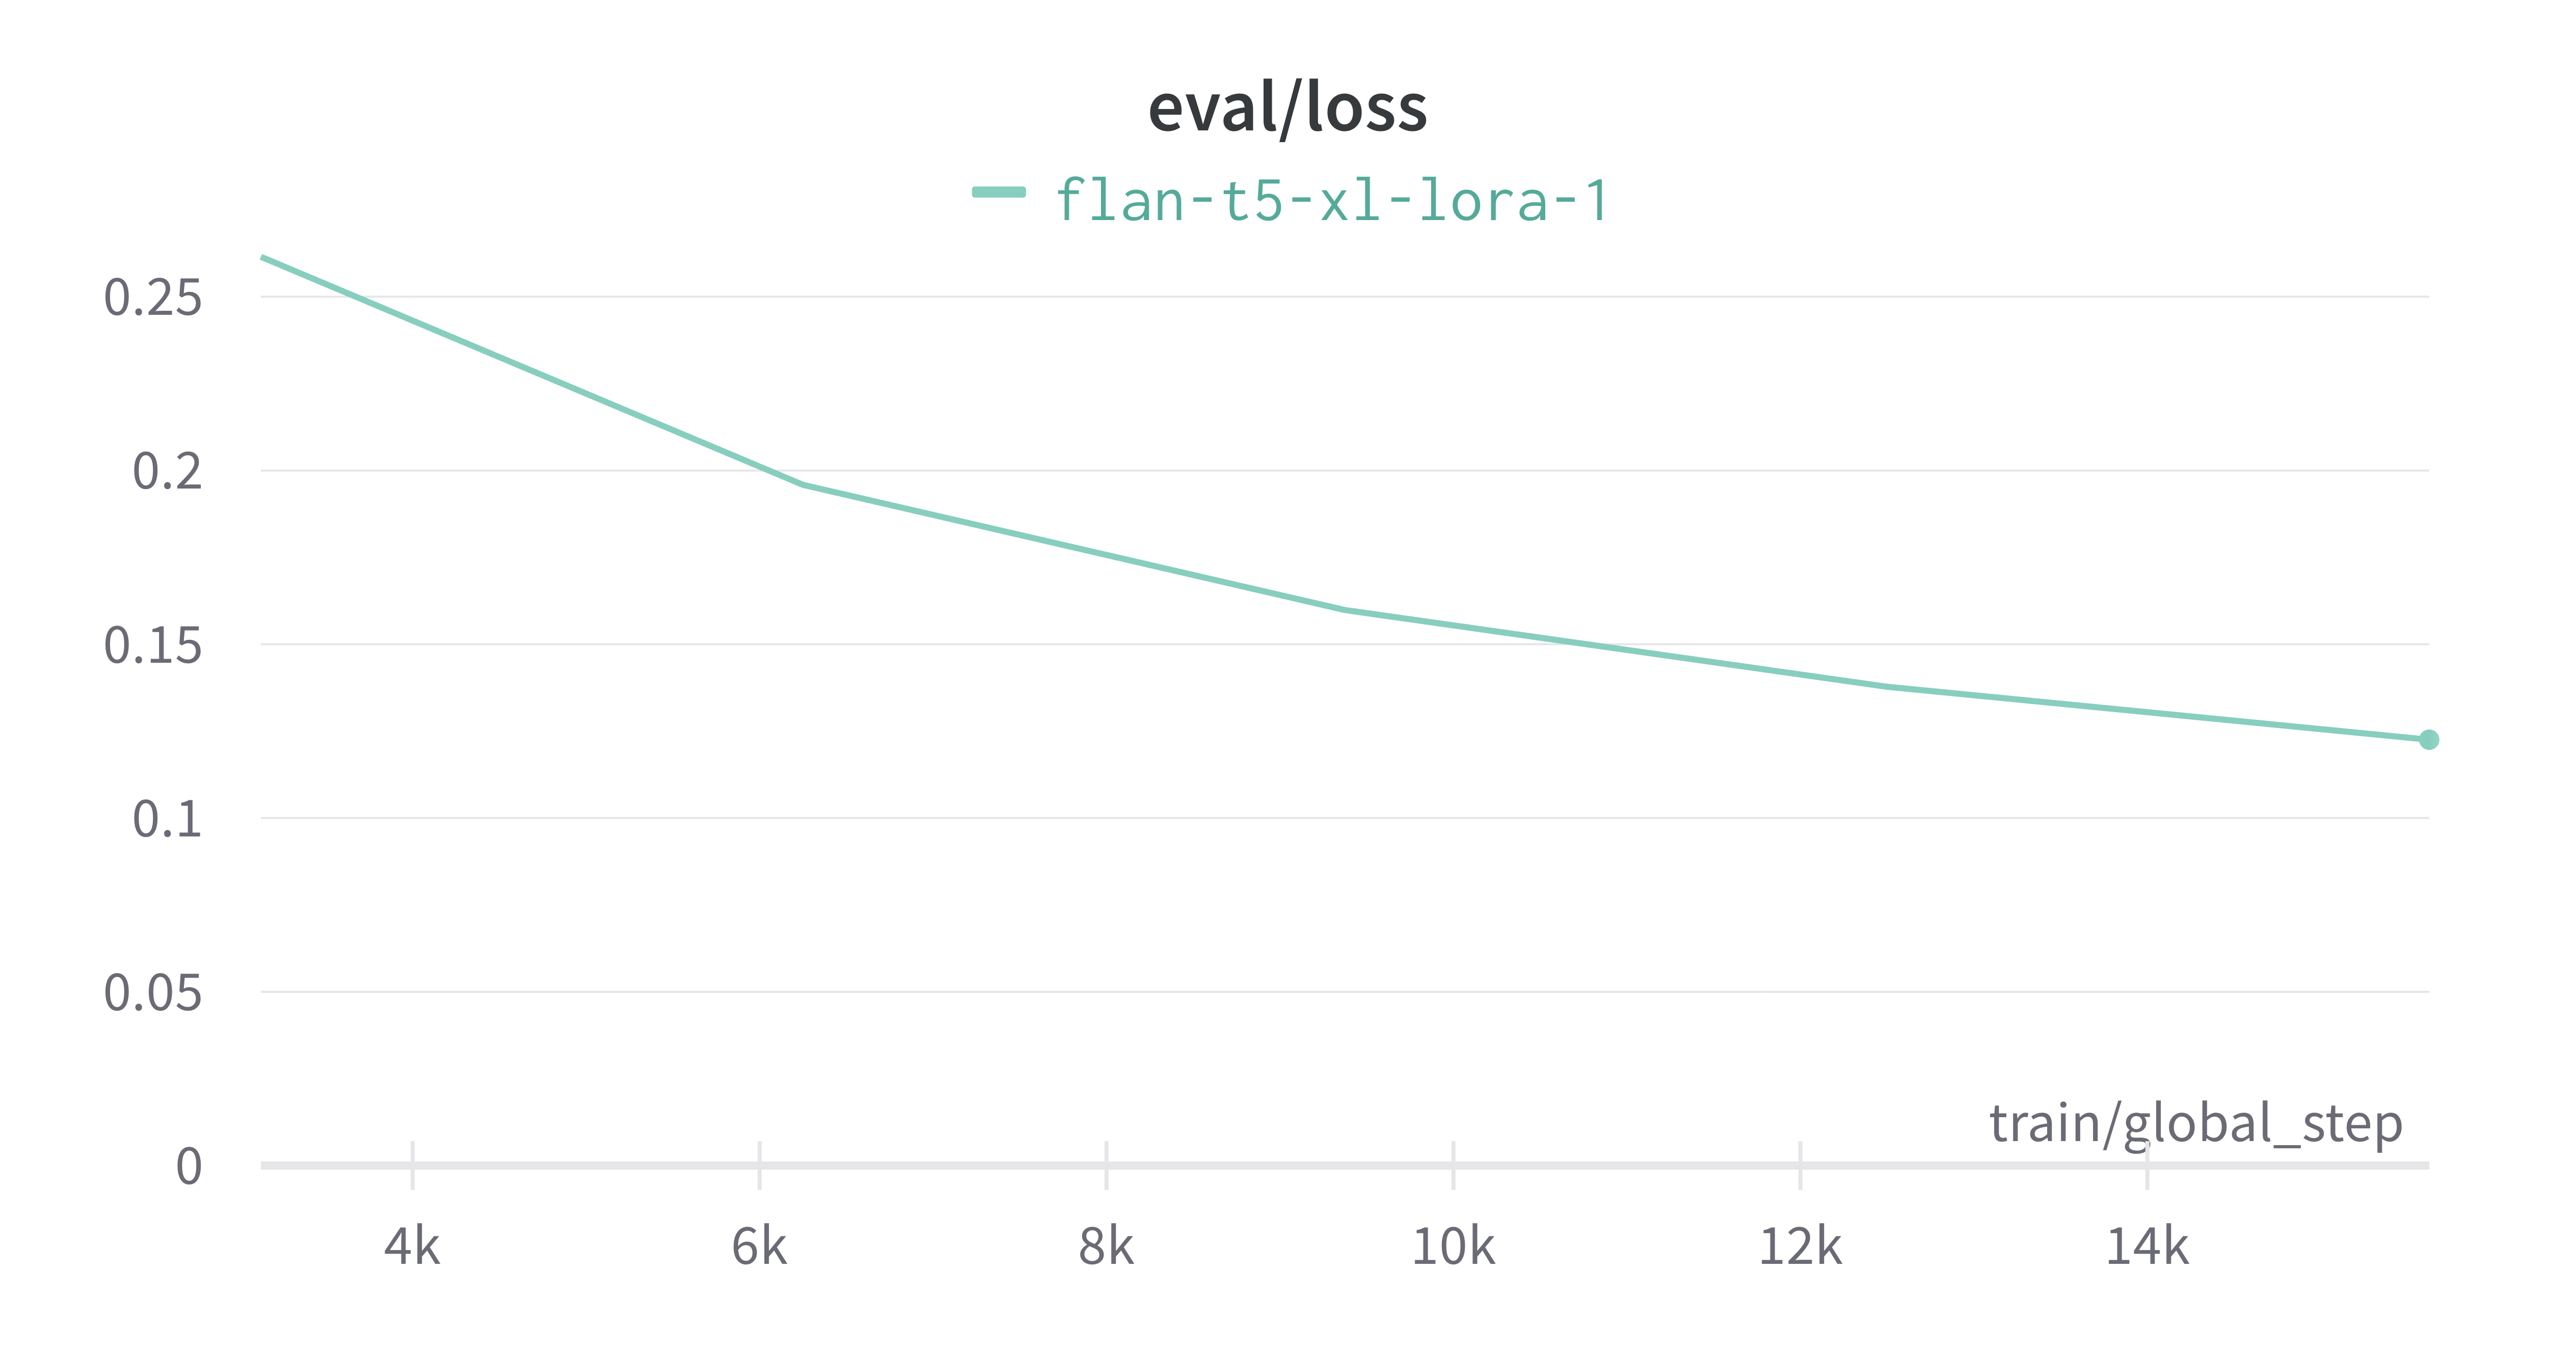
\includegraphics[width=.6\textwidth]{total-eval-loss}
  \caption{Значение функции ошибки на валидационных данных}
  \label{total-eval-loss}
\end{figure}

\begin{figure}[H]
  \centering
  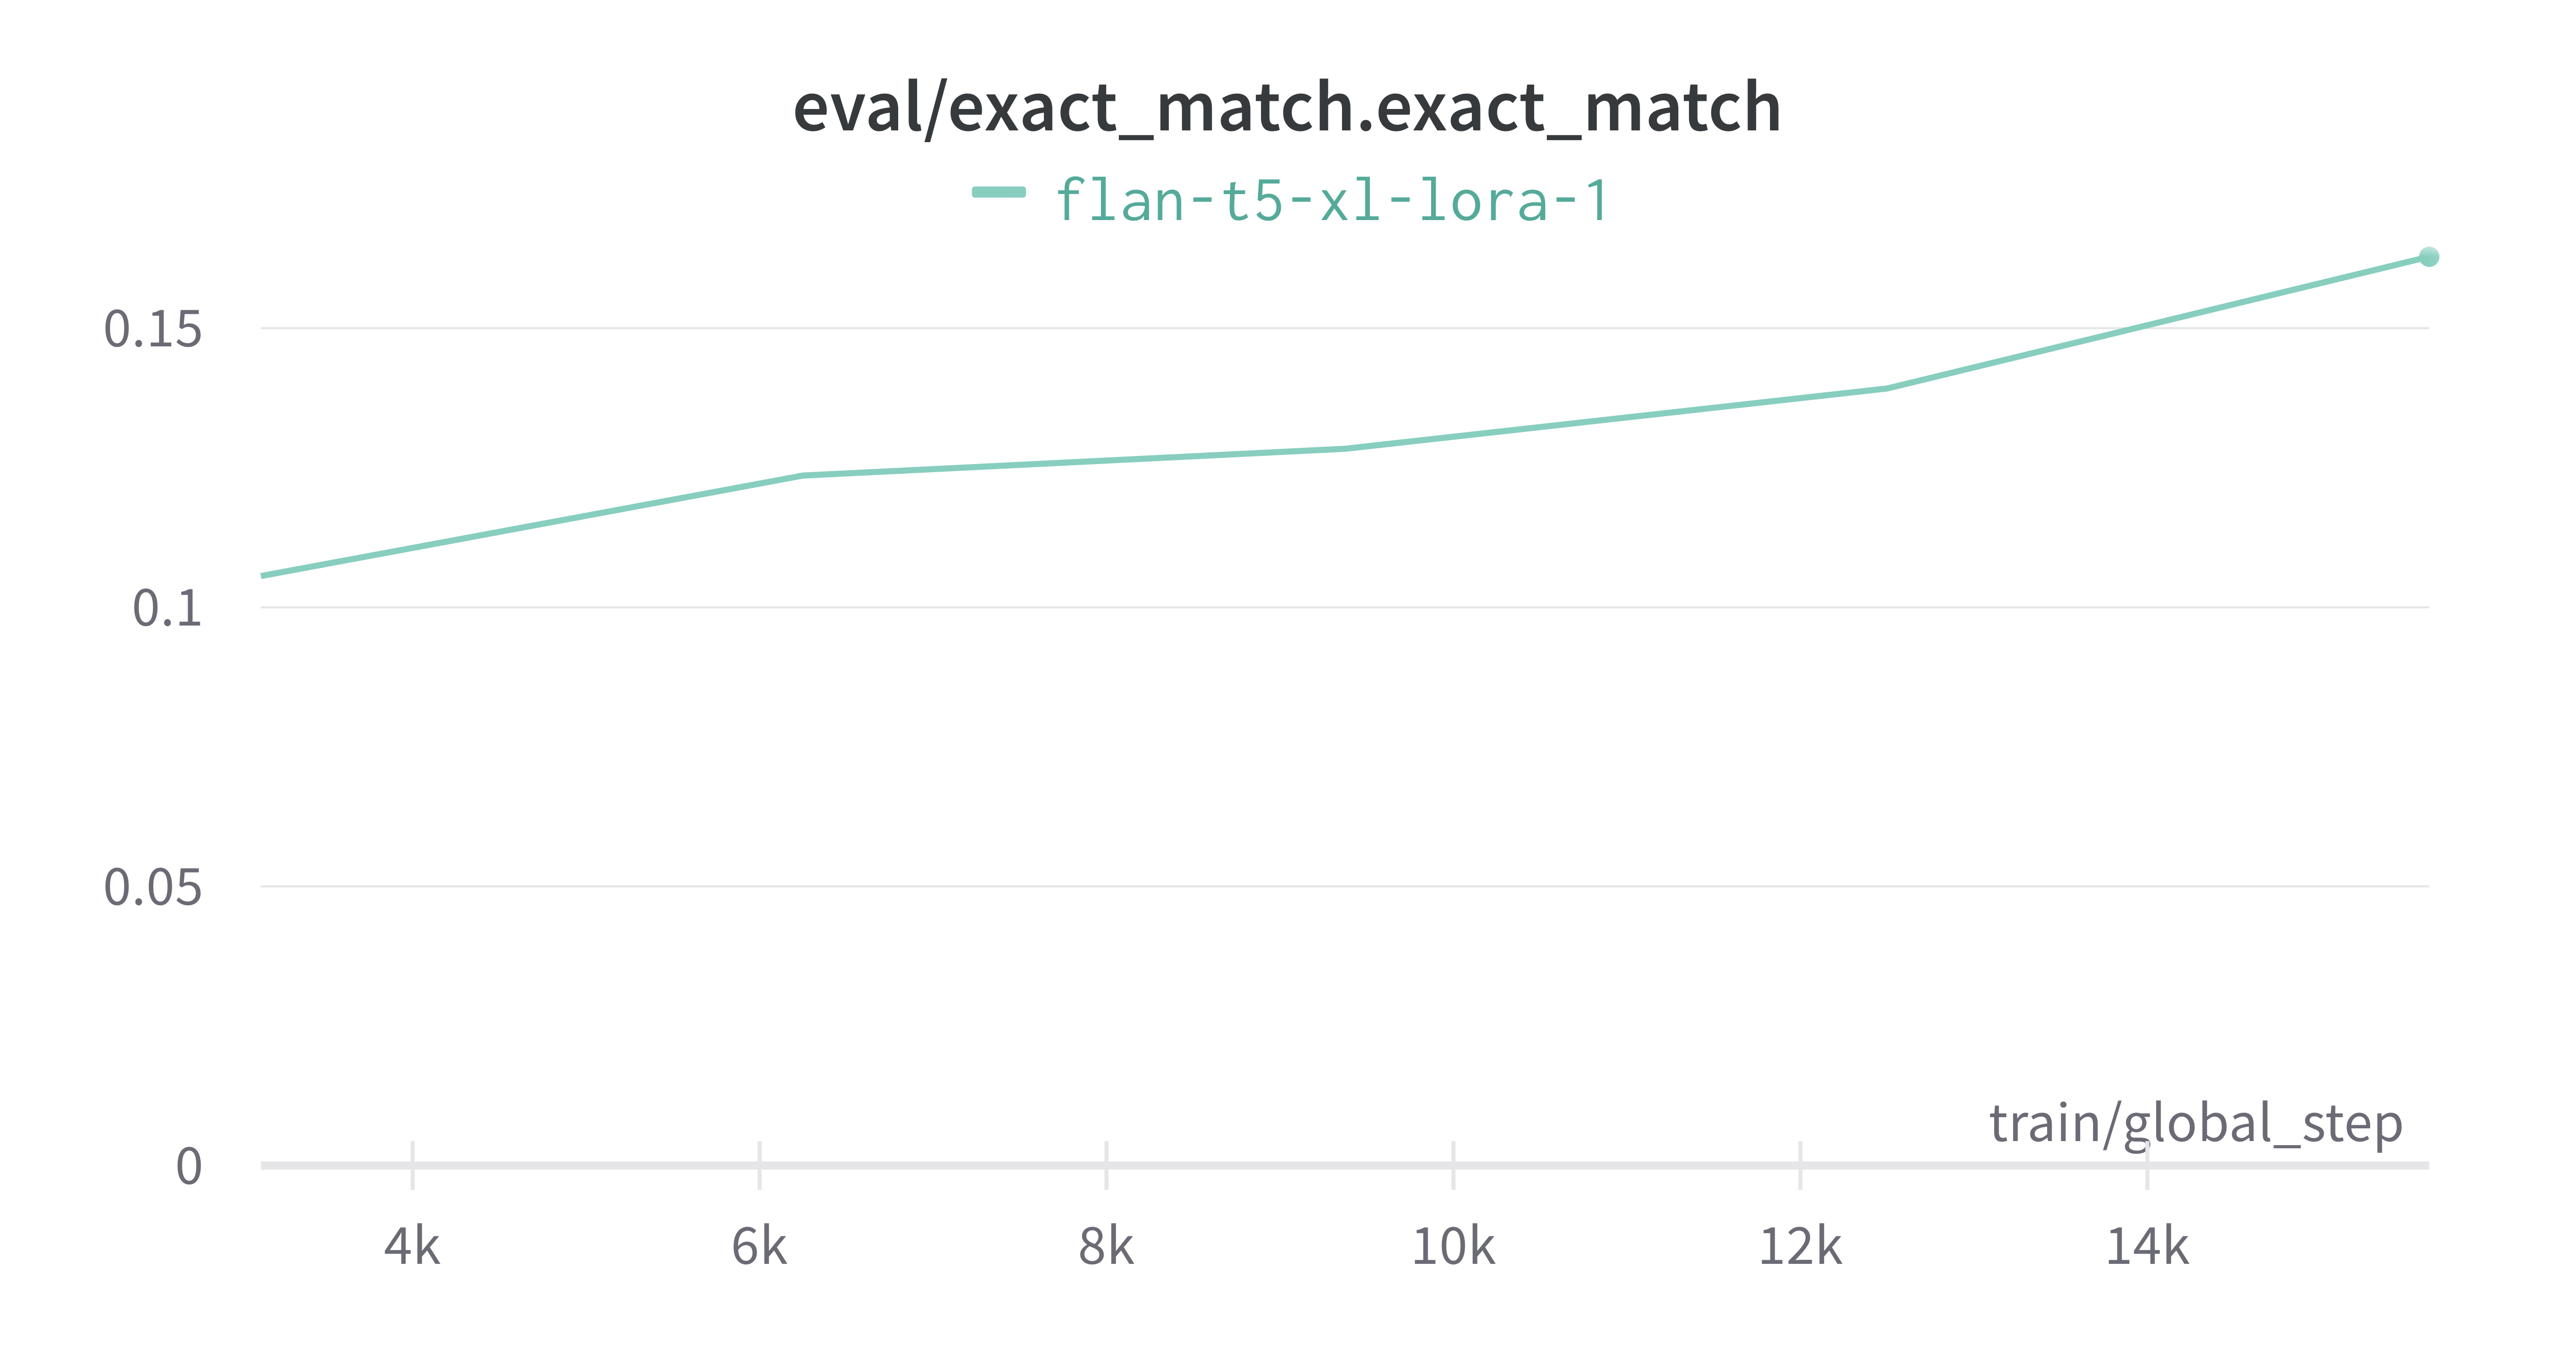
\includegraphics[width=.6\textwidth]{total-em}
  \caption{Значение метрики Exact Match на валидационных данных}
  \label{total-em}
\end{figure}

\begin{figure}[H]
  \centering
  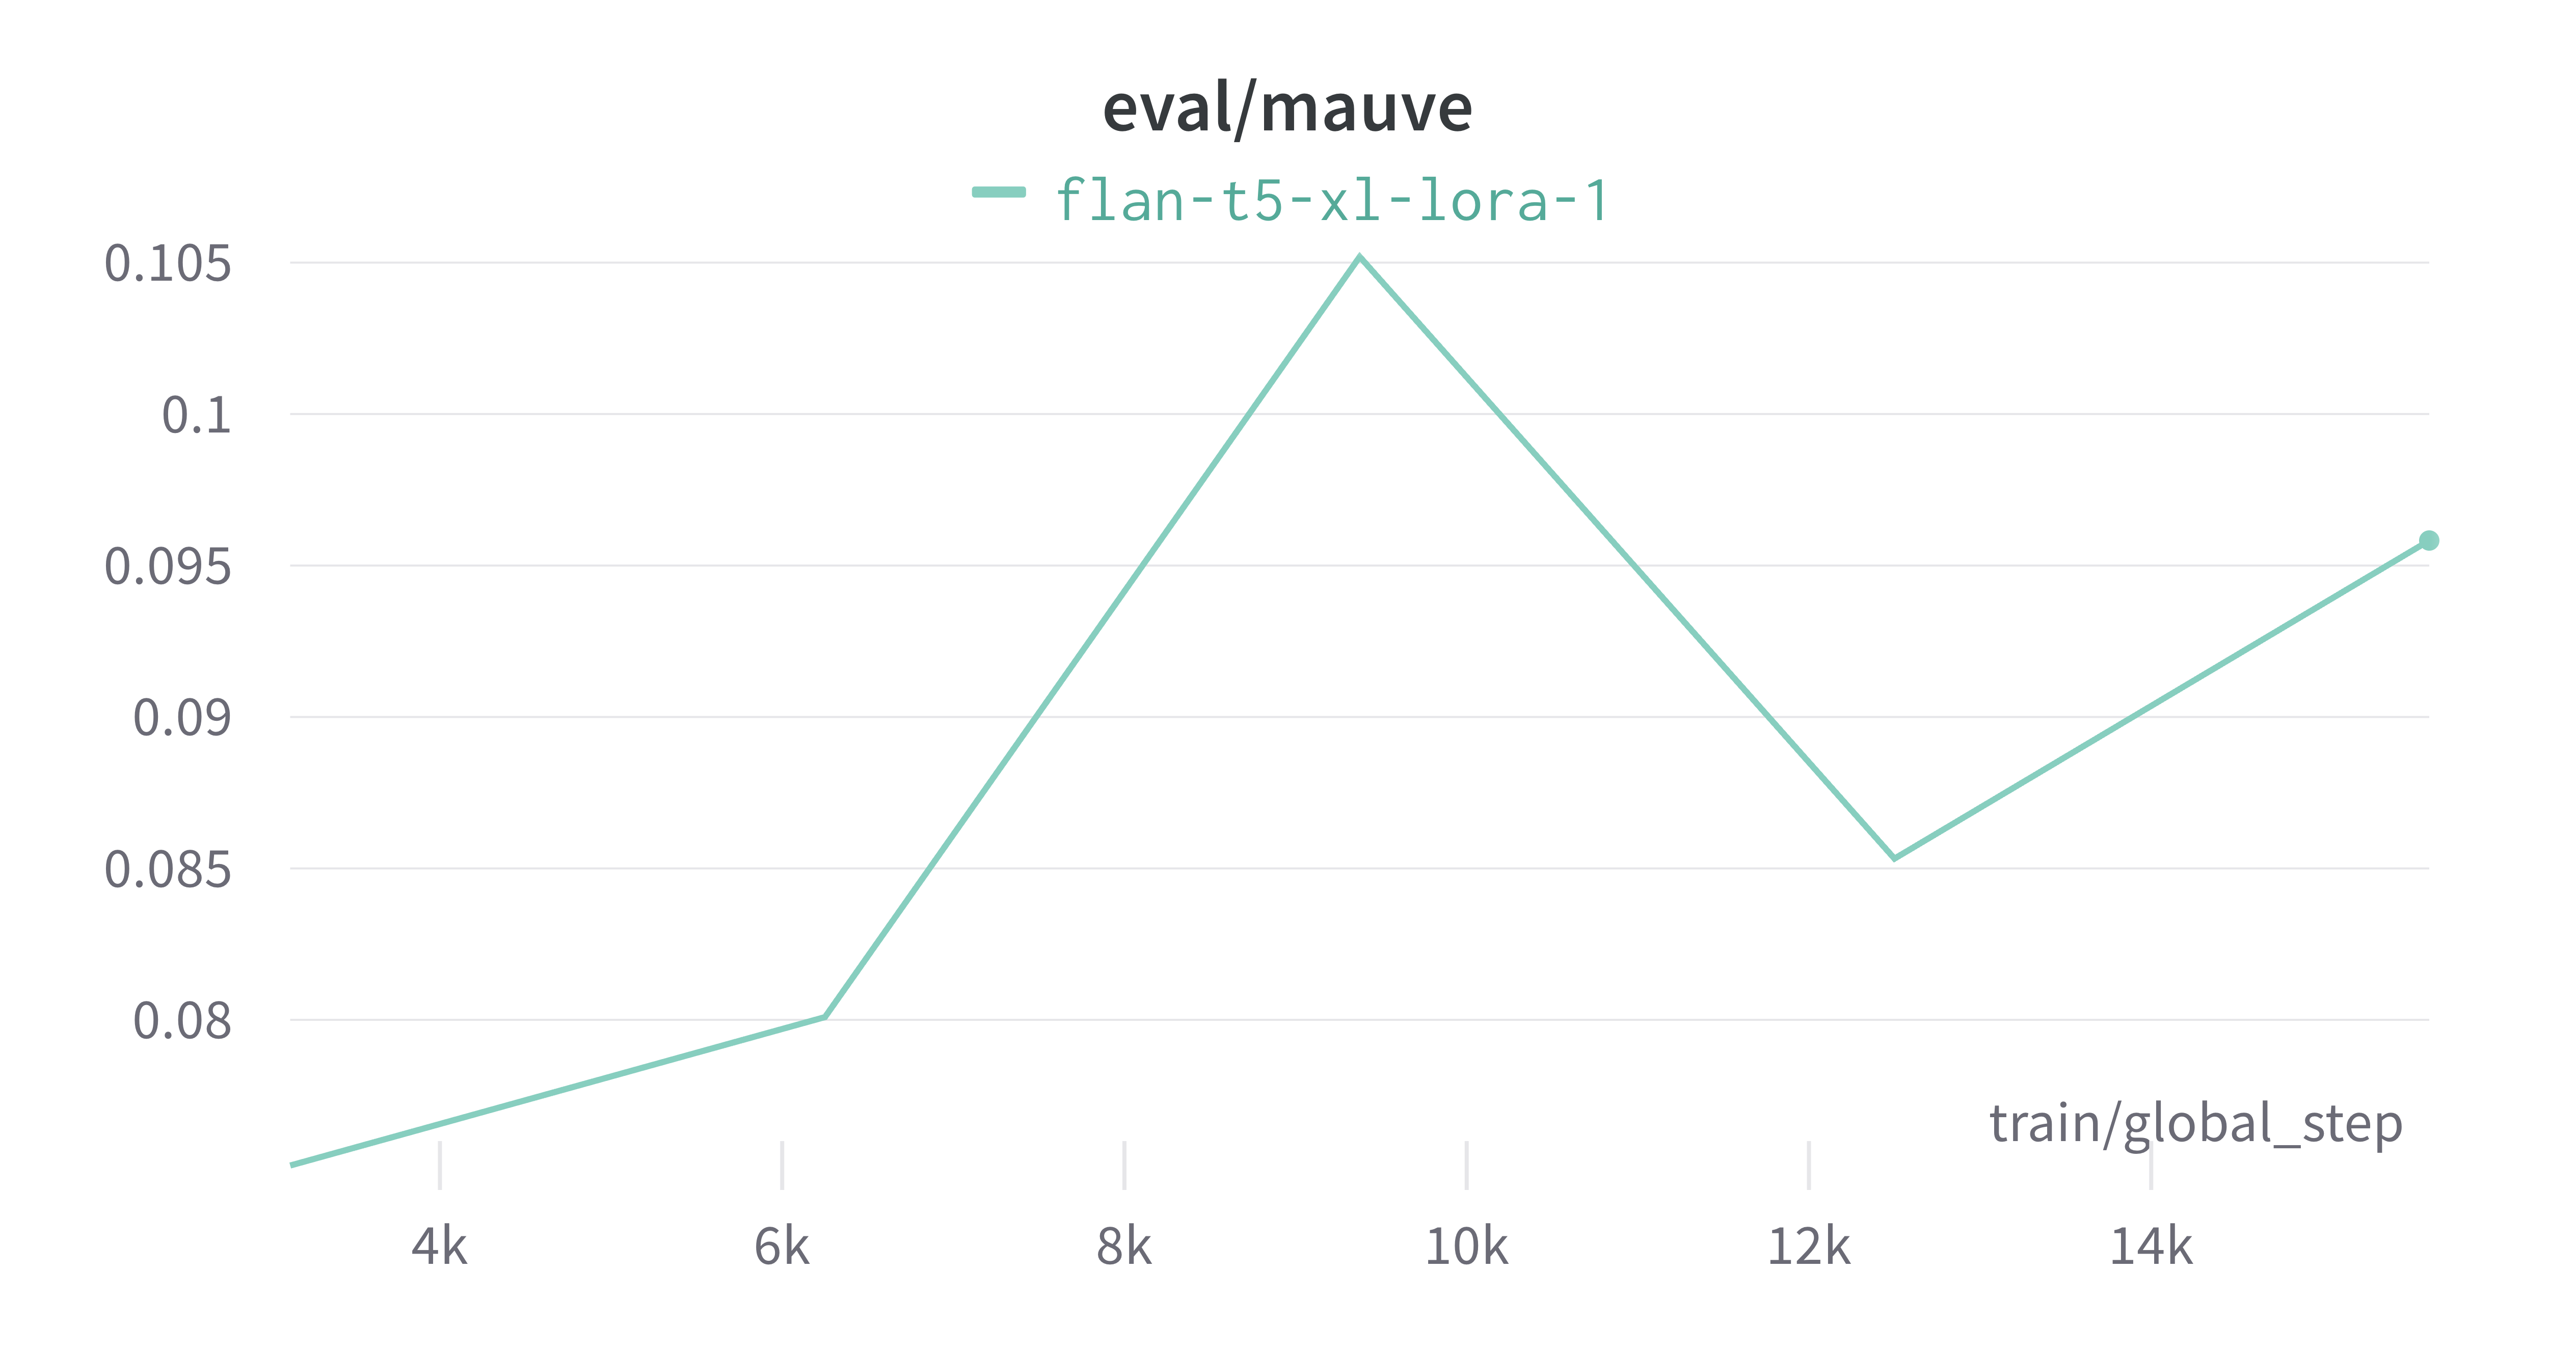
\includegraphics[width=.6\textwidth]{total-mauve}
  \caption{Значение метрики MAUVE на валидационных данных}
  \label{total-mauve}
\end{figure}
